\documentclass[tikz,border=10pt]{project_plan}
\usepackage[utf8]{inputenc}
\usepackage{selinput}
\usepackage{graphicx, subcaption, float}
\usepackage{hyperref}
\usepackage{cite}
\usepackage{ upgreek, amsmath, tipa , textcomp, amssymb  }
\usepackage{listings}
\usepackage{caption, wrapfig, lstautogobble}
\usepackage{ marvosym }
\usepackage[linguistics]{forest}
\usepackage{mdframed}
\usepackage[dvipsnames]{xcolor}
\mdfdefinestyle{MyQuoteFrame}{%
linecolor=blue,
rightline=false, topline=false, bottomline=false,
outerlinewidth=0.1pt,
innerleftmargin=3em,
backgroundcolor=white}

\newcommand{\sectionbreak}{%
\begin{center}
  % $\ast$~$\ast$~$\ast$
  \noindent\rule{8cm}{0.4pt}
\end{center}
}

\newcommand{\bulletPoint}{\hspace{-3.1pt}$\bullet$ \hspace{5pt}}
\setcounter{tocdepth}{7}

%---

\def\studentname{Faeq}
\def\projecttitle{Security Management}

%---

\begin{document}
\chapter*{What is Taught}

Notes for the Data Protection guest lecture were made but they are not examinable

Unit 6 was never covered and is not examinable

The guest lecture "John Randell's daily tasks" \colorbox{Thistle}{\textit{is} examinable}

\begin{itemize}
  \item Unit 1 - Introduction
        \begin{itemize}
          \item Definitions of risk assessments, Risk, security, security violation,
                vulnerability, threat, attacker, insider, script kiddies, explorer,
                cyber criminals, hacktivists, cyber terrorists, nation states, commercial
                spies, the CIA triad (confidentiality, integrity and availability),
                reliability, authenticity, accountability, non-repudiation, privacy,
                Information security management, ISMS, CISO
          \item The main types of security violations \& the 4 possibilities
          \item The capabilities and motivation of all attackers
          \item The security objectives of an ISMS \& its components
        \end{itemize}
  \item Unit 2 - Standards and Best Practices for Information Security Management
        \begin{itemize}
          \item Definitions of standard, framework, regulation, best practices
          \item The categories of standards
          \item What the ISO/IEC 27000-series is \& the structure
          \item The main parts of ISO/IEC 27000, its definition of and principles for a ISMS
          \item ISO/IEC 27001 overview \& the 7 main clauses
          \item What ISO/IEC 27002, ISO/IEC 27006, PCI-DSS \& Cyber essentials are
        \end{itemize}
  \item Unit 3 - Risk
        \begin{itemize}
          \item The ISO/IEC 31000 and ISO/IEC 27005 definitions of Risk \& the definition of risk culture
          \item The finance and cyber risk domains
          \item Ways of listing risks; Joe's way, STRIDE, PASTA
          \item Ways of assessing risk likelihood \& impact; DREAD, subjective/objective
          \item The different risk treatment options
        \end{itemize}
  \item Unit 4 - Security Controls
        \begin{itemize}
          \item Definitions of security control, operational capability, security policy
          \item The ways of viewing controls
          \item The ISO/IEC 27002 controls \& their categories (4 organizational, 4 physical, 5 technical)
          \item The different levels of security policies \& the communication and review of them
        \end{itemize}
  \item Unit 5 - Incident Management and Disaster Recovery
        \begin{itemize}
          \item Definitions of incident management, event, incident, incident response teams, business continuity, business continuity plan, disaster recovery
          \item The different plans for security events and incidents
          \item The phases of managing an incident
          \item Learning from incidents \& response procedures
          \item Documentation and testing of plans \& outsourcing
          \item The 1-2 punch; insiders, script kiddies, cyber criminals \& nation states, hacktavists \& terrorists
        \end{itemize}
  \item Unit 7 - Law \& Ethics
        \begin{itemize}
          \item Definitions of lead generation, marketing, spam, PII, PII controller, PII processor, pseudonymization, ethics
          \item Marketing, collecting data \& the notion of information wanting to be free
          \item GDPR \& it's principles and effects; ”Lawyers Provide Sound Advice In Data Affairs"
          \item The rights of individuals under GDPR
          \item Obligations for PII controllers \& processors
          \item Diversity as a defense
        \end{itemize}
  \item Guest lecture - John Randell's daily tasks
        \begin{itemize}
          \item The sort of questions he gets asked in tickets
          \item Evaluating risky sign ins
          \item The uses of SentinelOne for endpoint management
          \item Information provided by \& actions you can take in Microsoft Defender
          \item Analyzing reported emails; SPF, SKIM \& DMARC
          \item Finding suspicious or potentially malicious Outlook rules (Audit)
        \end{itemize}
  \item Unit 8 - Staff Management
        \begin{itemize}
          \item The 2 controls for before employment;
                \begin{itemize}
                  \item Screening; 5 basic checks \& 4 levels of DBS checks
                  \item Terms \& conditions of employment; what contracts \& job descriptions should include
                \end{itemize}
          \item The 5 controls during employment
                \begin{itemize}
                  \item Disciplinary process
                  \item Confidentiality; NDAs \& Security theatre
                  \item Awareness, education \& training
                  \item Remote working; asking what is really required \& email
                  \item Event reporting
                \end{itemize}
          \item The (1) control at the end of employment
                \begin{itemize}
                  \item Responsibilities after termination or change of employment; removing access
                \end{itemize}
        \end{itemize}
  \item Unit 9 - Audit
        \begin{itemize}
          \item The definitions of an audit, Risk homeostasis / compensation
          \item Internal \& External audits
          \item The ISO 27001 audit; stages, outcomes \& skepticism
        \end{itemize}
\end{itemize}

\newpage

\tableofcontents\pdfbookmark[0]{Table of Contents}{toc}\newpage

\chapter{Unit 1 - Introduction}

\section{Risk assessments}
\colorbox{green}{Risk assessments} are a \colorbox{yellow}{list of things that can go wrong}; how \colorbox{yellow}{likely}?, \colorbox{yellow}{how bad} if they happened?\\
Add \colorbox{yellow}{mitigation strategies} \& then revise scores for likelihood \& impact;

\colorbox{green}{Risk} = \colorbox{yellow}{likelihood * impact}

They are a way of \colorbox{pink}{making sure that you are worrying about the right thing} \& that you are \colorbox{pink}{doing something about it}

\begin{figure}[H]
  \centering
  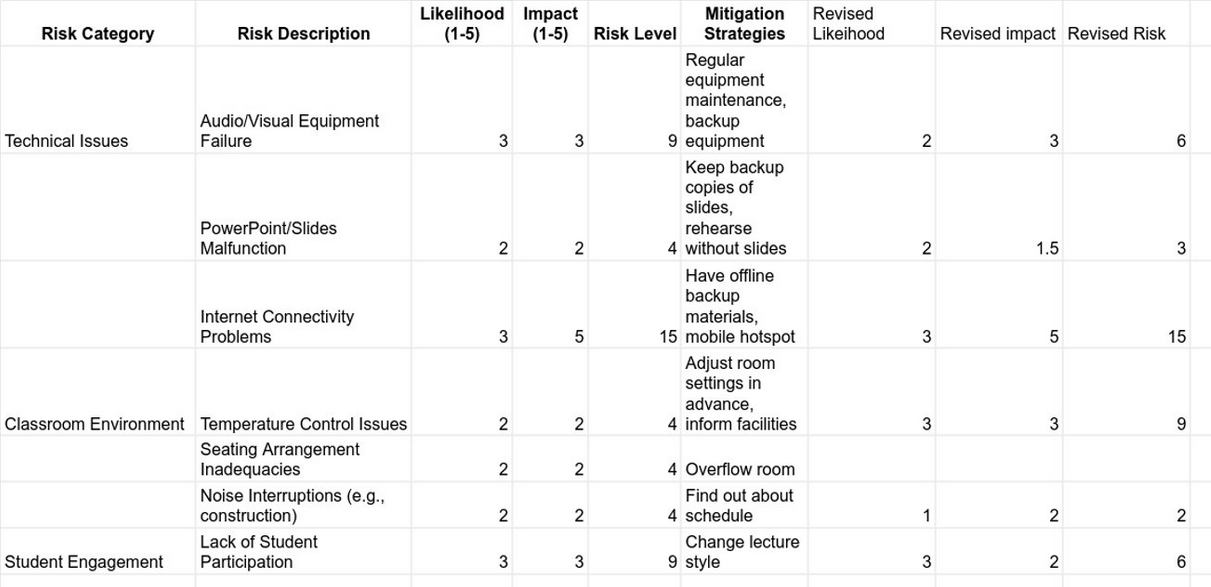
\includegraphics[width=\linewidth]{risk assessment.png}
  \caption{An example of a risk assessment for a lecture}
\end{figure}

\section{Security}

\colorbox{green}{Security} - The \colorbox{yellow}{measures put in place to protect an organization's assets}

\colorbox{green}{Security Violation} - \colorbox{yellow}{Damage done to a system/asset in some way}

Three \colorbox{cyan}{main types} (James Anderson 1972):\\
\bulletPoint Unauthorized \colorbox{pink}{information release}\\
\bulletPoint Unauthorized \colorbox{pink}{information modification}\\
\bulletPoint Unauthorized \colorbox{pink}{denial of use}

\newpage

4 \colorbox{cyan}{possibilities}:\\
\bulletPoint \colorbox{green}{Safe} - \colorbox{yellow}{Only the user has access},\\
\bulletPoint \colorbox{green}{Loss}  -\colorbox{yellow}{ No one has access},\\
\bulletPoint \colorbox{green}{Leak} - \colorbox{yellow}{Both the user and the adversary have access}, or\\
\bulletPoint \colorbox{green}{Theft} - \colorbox{yellow}{Only the adversary has access}

\colorbox{green}{Vulnerability}\\
A \colorbox{yellow}{flaw} or weakness in the design or \colorbox{yellow}{implementation of a system} that \colorbox{yellow}{could lead to a}
\colorbox{yellow}{security violation}, e.g., Program bugs, Misuse of system features, Configuration errors, Insecure designs

\colorbox{green}{Threat}\\
A \colorbox{yellow}{potential danger} or circumstance that can \colorbox{yellow}{exploit a vulnerability} in a system leading to a
\colorbox{yellow}{security violation}, e.g., a casual attacker running the same exploit script against all servers finds
yours hasn't patched the bug.

The \colorbox{pink}{threat sentence};\\
The exploit/attack exploits the vulnerability to cause a security violation\\
(The threat is the whole sentence)


\section{Attackers}
An \colorbox{green}{Attacker} is an \colorbox{yellow}{active opponent} who \colorbox{yellow}{takes advantage of vulnerabilities}; There are many types of attackers
Each kind of attacker has its own capabilities and motivation

Attackers are \colorbox{pink}{contextual}; GCHQ might consider someone a script-kiddie, but RHUL might think they are
a sophisticated cyber-criminal

\subsection{Insiders}
Persons with \colorbox{yellow}{legitimate access} to the organization\\
\bulletPoint Employees\\
\bulletPoint Third parties\\
\bulletPoint Contractors

Insiders are a huge threat in practice but are \colorbox{pink}{very difficult to defend against}\\
\colorbox{pink}{Not all} insiders are \colorbox{pink}{malicious} but many are careless

Capabilities:\\
\bulletPoint Already have access to the organization\\
\bulletPoint May depend on the role

Motivation:\\
\bulletPoint Not necessary\\
\bulletPoint Lack of motivation can be risky\\
\bulletPoint But disgruntled employees can cause a lot of harm

\subsection{Script Kiddies}

People who \colorbox{yellow}{use other tools} or scripts \colorbox{yellow}{to perform attacks}\\\\
Capabilities\\
\bulletPoint Generally, \colorbox{pink}{not technically knowledgeable}

Motivation\\
\bulletPoint Curiosity\\
\bulletPoint Money

\subsection{Explorer}
People \colorbox{yellow}{capable of developing tools} and scripts \colorbox{yellow}{to perform attacks}\\\\
Capabilities\\
\bulletPoint Good technical skills

Motivation
\begin{itemize}
  \item Fame
  \item Money
        \begin{itemize}
          \item Hack for hire
          \item Red teams
        \end{itemize}
\end{itemize}

\subsection{Cyber Criminals}
\colorbox{yellow}{Organizations} that carry out \colorbox{yellow}{criminal activities} with a \colorbox{yellow}{electronic element}\\\\
Capabilities\\
\bulletPoint Wide range\\
\bulletPoint Outsourcing of tools and development

Motivation
\begin{itemize}
  \item Money
        \begin{itemize}
          \item Ransomware
          \item Credit card fraud
        \end{itemize}
\end{itemize}

\subsection{Hacktivists}
\colorbox{yellow}{Activists} that perform their operations \colorbox{yellow}{on the Internet} (e.g. Anonymous)\\\\
Capabilities
\begin{itemize}
  \item Very heterogeneous groups
        \begin{itemize}
          \item Media experts
          \item Technical experts
          \item Political experts
          \item Journalists
        \end{itemize}
  \item Sometimes disorganized
\end{itemize}

Motivation\\
\bulletPoint Political in most cases

Difference between hacktivist groups and multiple script-kiddies; \colorbox{pink}{agenda}

\subsection{Cyber terrorists}
A person who \colorbox{yellow}{uses unlawful violence} and intimidation, especially against civilians,
in the pursuit of \colorbox{yellow}{political aims}.

Terrorist that use computers as a means of attack (e.g. Anonymous)

Capabilities\\
\bulletPoint Not knowledgeable enough (at the moment)

Motivation\\
\bulletPoint Political motivations

Although terrorist groups use the internet as a recruitment tool this is not generally
considered as cyber terrorism

\subsection{Nation States}
\colorbox{yellow}{States} that carry out \colorbox{yellow}{information warfare operations}\\\\
Capabilities\\
\bulletPoint Technically and financially supported by Intelligence Agencies

Motivation\\
\bulletPoint Political; e.g., Stuxnet

\subsection{Commercial Spies}
From Wikipedia:\\
While political espionage is conducted or orchestrated by governments and is
international in scope, industrial or corporate espionage is more often national
and occurs between \colorbox{pink}{companies} or corporations

In practice, this is more a \colorbox{pink}{social threat} than a cyber threat

Vastly increased labour mobility means that the easy way of finding out what your competitor is doing is to hire one of
their employees and ask them

But this heavily overlaps with nation-state attackers

\section{Security Goals}

It is unfortunate that these security goals are inconsistently defined even within organisations who exist to produce consistent standards.
As ever, “Security is what your boss says it is”

\colorbox{green}{CIA triad};\\
Confidentiality - Unauthorised information release\\
Integrity - Unauthorised information modification\\
Availability - Unauthorised denial of use

We must always \colorbox{pink}{analyse CIA in the context} of the business needs

There are additional possible security goals;\\
\bulletPoint Accountability\\
\bulletPoint Reliability\\
\bulletPoint Non-repudiation\\
etc.

\subsection{Confidentiality}
\bulletPoint Information can \colorbox{yellow}{only be read by authorised parties}\\
\bulletPoint Prevention of unauthorised information release

Confidentiality is sometimes confused with security; this is not true\\
This is just one property of security

E.g.\\
Messages sent through WhatsApp\\
End-to-end encrypted between senders\\
Facebook does not know the content of our messages, but they know who we talk with

E.g.\\
How do we ensure that a lost device doesn't compromise an organisation's confidential data?\\
Full and File-based disk encryption

\subsection{Integrity}
\bulletPoint Information can \colorbox{yellow}{only be modified by authorised parties}\\
\bulletPoint Prevention of unauthorised information modification

Several definitions \colorbox{pink}{depending on context};\\
Computing: Preventing unauthorised writes of information\\
- Tampering with data \\
Systems: Prevent unauthorised changes of the system\\
- Tampering with a system \\
Communications: Detect and correct of modification of transmitted data\\
- Avoid changes of data sent through a public channel

Integrity is \colorbox{pink}{often a prerequisite} for other security properties

E.g.\\
Application development - Second-factor authentication, Signed commits

E.g.\\
Blockchain in Bitcoin\\
\bulletPoint Goal: accurate record of all transactions\\
\bulletPoint All transactions are signed and recorded in the blockchain\\
\bulletPoint It is almost impossible to tamper the blockchain (need more than 51\% of the network in control)

\subsection{Availability}
Information can be \colorbox{yellow}{accessed when needed} by \colorbox{yellow}{authorized entities}\\
Prevention of unauthorised denial of use

Not only a security property; requires \colorbox{pink}{fault-tolerance}

In security we are concerned with avoiding Denial of Service (DOS)\\
\bulletPoint Accidental\\
\bulletPoint Deliberate

E.g.\\
Mirai botnet\\
\bulletPoint Botnet of IoT devices used to attack websites\\
\bulletPoint Initially used to DDoS Minecraft\\
Ransomware attacks\\
\bulletPoint Malware that encrypts victim's files, so they are unreadable

\subsection{Other security goals}

\subsubsection{Reliability}
The system must perform properly even in adverse conditions;\\
\colorbox{yellow}{consistent intended behaviour and results}\\
\colorbox{pink}{System testing} is a fundamental process for this property

Best examples\\
\bulletPoint Nuclear power plants\\
\bulletPoint Planes\\
\bulletPoint Netflix

\subsubsection{Authenticity}
Property that an \colorbox{yellow}{entity is what it claims to be}.

Normally easy for an individual and quite hard for an organization\\
Hard for individuals sometimes; relies on authenticating organisations

\subsubsection{Accountability}

We cannot prevent security violations\\
Accountability helps dealing with security breaches\\
\bulletPoint Trace system misuse by users\\
\bulletPoint Detect breaches and anomalous behaviour

How?\\
\bulletPoint Securely identifying users\\
\bulletPoint Keep record of actions of each User

\subsubsection{Non-repudiation}
The ability to \colorbox{yellow}{prove the occurrence} of a claimed \colorbox{yellow}{event} or action \colorbox{yellow}{and its originating entities}

It is a legal term, borrowed by security. \\
In essence “Can a user deny having sent a message” or “Can a user deny having purchased something”

Most sources treat non-repudiation and accountability as the same thing used in a mildly different context.\\
But \colorbox{pink}{ISO 27000 lists them separately}, without defining one of them;\\
"non-repudiation or accountability: the ability of a system to confirm that a sender cannot convincingly deny having sent something".

General differences: \\
\bulletPoint Non-repudiation is used more in external contexts\\
\bulletPoint Non-repudiation is used more in legal contexts\\
\bulletPoint Non-repudiation is used more in very technical IS.\\
\bulletPoint Non-repudiation is slightly more likely to be used for a single message.

For the purposes of this course:\\
\colorbox{green}{Non-repudiation} is a \colorbox{yellow}{specific type of accountability} related to \colorbox{yellow}{contracts and agreements} rather than general logging that that might be used to diagnose problems.

\subsubsection{Privacy}
An orthogonal goal

Privacy is not confidentiality nor security\\
\colorbox{green}{Privacy} is the \colorbox{yellow}{protection of} Personally Identifiable Information (\colorbox{yellow}{PII}) \colorbox{yellow}{from misuse}

This implies several things for an organisation;\\
\bulletPoint Give control of PII to owner\\
\bulletPoint Look after PII properly

\colorbox{pink}{Privacy is not security} but generally \colorbox{pink}{relies on the correct implementation of security measures}

\section{Information Security management}
All the aspects of making security happen in an organisation

\colorbox{green}{Information security management} -
\colorbox{yellow}{creating} a \colorbox{yellow}{risk-managed environment} so the \colorbox{pink}{organisation} \colorbox{pink}{can focus on achieving its business goals}.

\newpage

Information Security Management system (\colorbox{green}{ISMS}) -
the \colorbox{yellow}{system} (policies, processes, controls, etc.) put in place to \colorbox{yellow}{achieve} that \colorbox{yellow}{risk-managed environment}

The Chief Information Security Officer \colorbox{pink}{(CISO) is in charge of the ISMS}

Because the environment involves the organisation, ISMS needs to be traversal to the whole organisation and will \colorbox{pink}{impact all units within the organisation}

\subsection{Security objectives of an ISMS}

The highest levels are the \colorbox{pink}{CIA} but are \colorbox{pink}{too broad in practice}

The \colorbox{green}{goals} will need to be \colorbox{pink}{defined related to the assets and their criticality} to the organisation\\
\bulletPoint These are generally defined in terms of the \colorbox{pink}{risk the organisation wants to accept}\\
\bulletPoint They are developed as the \colorbox{yellow}{result of a risk assessment}

Components of an ISMS:\\
\bulletPoint Information Security\\
\bulletPoint IS Policies\\
\bulletPoint IS Organisation\\
\bulletPoint Management of Information Assets\\
\bulletPoint Human Resources\\
\bulletPoint Physical Security\\
\bulletPoint Communications and Operations\\
\bulletPoint Access Controls\\
\bulletPoint Compliance\\
\bulletPoint Business Continuity Management\\
\bulletPoint Incident Management\\
\bulletPoint IT acquisition, development and maintenance

\chapter{Unit 2 - Standards and Best Practices for Information Security Management}
A \colorbox{green}{standard} is an \colorbox{yellow}{agreed way of doing something}

Who produces standards?\\
\bulletPoint Private companies\\
\bulletPoint Consortiums\\
\bulletPoint Standardisation bodies\\
\bulletPoint Government

Standards establish a \colorbox{pink}{minimum set of requirements}; Good for doing the right thing\\
A Common baseline;  Good for resource planning and interoperability\\
Allow measurement and comparison between organisations\\
Marketing tool - can be necessary to get into a sector\\
e.g., PCI-DSS (Payment Card Industry – Data Security Standard)

Reading a standards document;\\
Bad people try hard to get the benefits without doing the work, and so the
standards documents end up being a long list of statements that close loopholes
that people have tried to exploit in the past.\\
It is useful for every unexpected statement, to imagine the circumstances
that required the rule.

Two \colorbox{cyan}{main categories}:\\
\bulletPoint \colorbox{green}{De facto}\\
\colorbox{yellow}{Widely used} in \colorbox{yellow}{specific area} but \colorbox{yellow}{not officially recognised}\\
Examples: Moodle, Office\\
\bulletPoint \colorbox{green}{De jure}\\
\colorbox{yellow}{Officially endorsed} by a body/government\\
Examples: HTML, ISO/IEC 27001\\
Can be \colorbox{pink}{auditable and certifiable} by the governing body

\colorbox{green}{Framework} -
A \colorbox{yellow}{structure, outline or process} which \colorbox{yellow}{supports an approach} to a specific objective\\
A framework is broad overview, outline, or skeleton of interlinked items, which \colorbox{pink}{serves as a guide}

Generally \colorbox{pink}{derived from standards}, and helps to implement standards\\
- generally \colorbox{pink}{assume good faith}, which standards might not

Examples:\\
NIST Cyber Security Framework

\colorbox{green}{Regulation} - a \colorbox{yellow}{binding legislative act}

\bulletPoint Regulations are \colorbox{pink}{formulated by Government} or administrative agencies with \colorbox{pink}{power to enforce law}\\
\bulletPoint Regulations are \colorbox{pink}{enforceable and auditable}\\
\bulletPoint Regulations could attract \colorbox{pink}{disciplinary actions} due to non-compliance

Examples:\\
GDPR

\colorbox{green}{Best Practices} - Set of \colorbox{yellow}{guidelines} that describe an \colorbox{yellow}{optimal way of doing things}

\bulletPoint Produced by many different organisations; Government, private sector, etc.\\
\bulletPoint Best practices may depend on the goal we want to optimise\\
\bulletPoint \colorbox{pink}{Auditable but non certifiable}

\section{ISO/IEC 27000 Series}
Published by ISO and IEC

ISO is the International Organization for Standardization\\
IEC is the International Electrotechnical Commission\\

ISO/IEC have a joint technical committee (JTC 1) that produces standards covering Information Technology

The 27000-series are produced by a subcommittee (SC 27)\\
SC 27 produces security standards

\colorbox{pink}{ISO is made up of national standards bodies};\\
BSI (UK), AFNOR (France), ANSI (US), DIN (Germany), JISC (Japan) …

ISO/IEC 27000 series dominates today’s world as the \colorbox{pink}{basis for ISM}\\
The series provides a \colorbox{cyan}{range of material}, including\\
\bulletPoint Definitions of basic terminology\\
\bulletPoint Descriptions of how to establish and operate an ISMS\\
\bulletPoint Detailed guidance on security controls and also on measuring their effectiveness\\
\bulletPoint Detailed guidance on risk assessment and security audit\\
\bulletPoint Sector-specific supplements

\newpage

Structure:\\
(darker ones are the ones to care about)\\
\begin{figure}[h!]
  \centering
  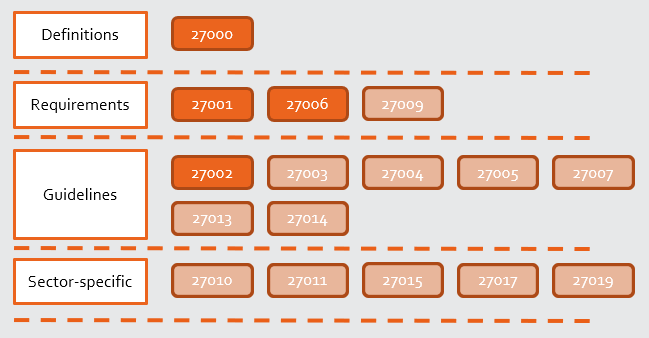
\includegraphics[width=\linewidth]{ISO_IEC_27000_series_structure.png}
\end{figure}

\subsection{ISO/IEC 27000}
The title of ISO/IEC 27000 is "Information security management systems – Overview and vocabulary".

ISO/IEC 27000 is \colorbox{pink}{descriptive}\\
\colorbox{yellow}{Describes the context and establishes terminology}

It sets remainder of 27000 series in context.\\
It has three \colorbox{cyan}{main parts}\\
\bulletPoint Definitions of fundamental ISMS terms\\
\bulletPoint Description of what constitutes an ISMS\\
\bulletPoint Description of each of the members of the ISO/IEC 27000 family

Defines an \colorbox{green}{ISMS} as Policies, processes, controls, etc. put in place to achieve a risk-managed environment\\
A \colorbox{yellow}{systematic approach} to\\
\bulletPoint establish\\
\bulletPoint implement\\
\bulletPoint operate\\
\bulletPoint monitor\\
\bulletPoint review\\
\bulletPoint improve\\
information security to meet business objectives

\newpage

\colorbox{cyan}{Principles} for a successful ISMS:\\
\bulletPoint \colorbox{pink}{Awareness of need} for information security\\
\bulletPoint \colorbox{pink}{Assigning responsibility} for information security\\
\bulletPoint Getting senior \colorbox{pink}{management commitment}\\
\bulletPoint Risk assessments \colorbox{pink}{determining appropriate controls}\\
\bulletPoint Security an essential element of information systems\\
\bulletPoint \colorbox{pink}{Active} prevention/detection of security incidents\\
\bulletPoint Continual reassessment

\subsection{ISO/IEC 27001}

ISO/IEC 27001 is \colorbox{pink}{definitive}\\
Sets down \colorbox{yellow}{standardised requirements} - It uses ‘shall’ and gives instructions\\
This allows organisations to claim compliance to ISO/IEC 27001 (and be \colorbox{pink}{audited} against it)

ISO/IEC 27001 is the \colorbox{pink}{key ISMS standard}.\\
Its provisions are therefore of key importance.

\colorbox{cyan}{Overview};\\
1. Establish the ISMS\\
2. Implement \& operate the ISMS\\
3. Monitor \& review the ISMS\\
4. Maintain \& improve the ISMS\\
5. GOTO 3

ISO/IEC 27001  contains seven main clauses (sections)\\
4. Context of the organisation\\
5. Leadership\\
6. Planning\\
7. Support\\
8. Operation\\
9. Performance evaluation\\
10. Improvement

It is potentially hugely helpful to have this ‘best practice’ encoded in such a way that organisations can be assessed for their compliance with best practice\\
The major shortcoming is that it \colorbox{pink}{does not prevent companies doing ‘just enough’} to comply\\
This is where ‘best practice’ comes in.

ISO/IEC 27001 approach involves performing many actions\\
\bulletPoint Risk assessment\\
\bulletPoint Selection and implementation of controls from 27002\\
There are a plethora of products designed to help with the process

\newpage

\subsubsection{Clause 4; Context}
\colorbox{yellow}{The organisation shall determine};\\
\bulletPoint \colorbox{yellow}{Interested parties} relevant to the ISMS\\
\bulletPoint \colorbox{yellow}{Requirements} of these interested parties\\
\begin{tabular}{r |@{\bulletPoint} l}
   & Legal and regulatory    \\
   & Contractual obligations \\
\end{tabular}\\
\bulletPoint The \colorbox{yellow}{boundaries} and applicability of the ISMS\\
\bulletPoint The \colorbox{yellow}{context} shall be documented (due to continual improvement requirement)

The \colorbox{pink}{scope} must be documented;
\begin{figure}[h!]
  \centering
  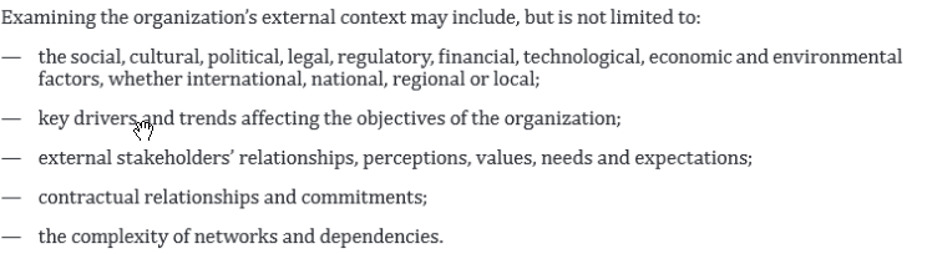
\includegraphics[width=\linewidth]{27001_clause4_context_1.png}
  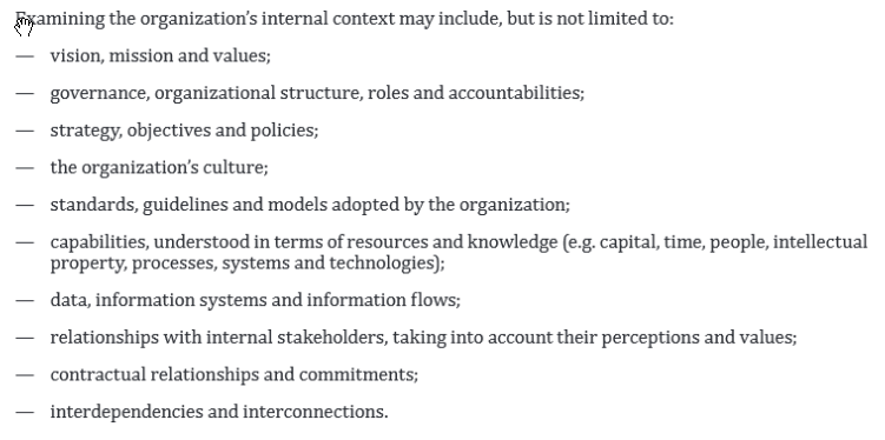
\includegraphics[width=\linewidth]{27001_clause4_context_2.png}
\end{figure}

\newpage

\subsubsection{Clause 5; Leadership}
\colorbox{yellow}{Top management shall};\\
\bulletPoint \colorbox{yellow}{Demonstrate commitment} with respect to the ISMS\\
\begin{tabular}{r |@{\bulletPoint} l}
   & Ensuring information security objectives are set and are compatible with the strategic direction \\
   & Ensuring resources needed for the ISMS are available                                             \\
\end{tabular}\\
\bulletPoint Ensure that the \colorbox{yellow}{responsibilities and authorities} for roles relevant to information security are \colorbox{yellow}{assigned and communicated}\\ (in general, you can replace ‘information security in that sentence with any business function)\\
\bulletPoint \colorbox{yellow}{Establish an information security policy}\\
\begin{tabular}{r |@{\bulletPoint} l}
   & Is \colorbox{yellow}{appropriate} to the purpose of the organisation                            \\
   & Includes information security \colorbox{yellow}{objectives}                                     \\
   & includes a \colorbox{yellow}{commitment} to satisfy applicable requirements related to security \\
   & Includes a commitment to continual improvement of the ISMS                                      \\
\end{tabular}\\
\bulletPoint The information security policy shall\\
\begin{tabular}{r |@{\bulletPoint} l}
   & be \colorbox{yellow}{available} as documented information;      \\
   & be \colorbox{yellow}{communicated} within the organisation; and \\
   & be available to interested parties, as appropriate              \\
\end{tabular}\\

Security Policy example;
\begin{figure}[h!]
  \centering
  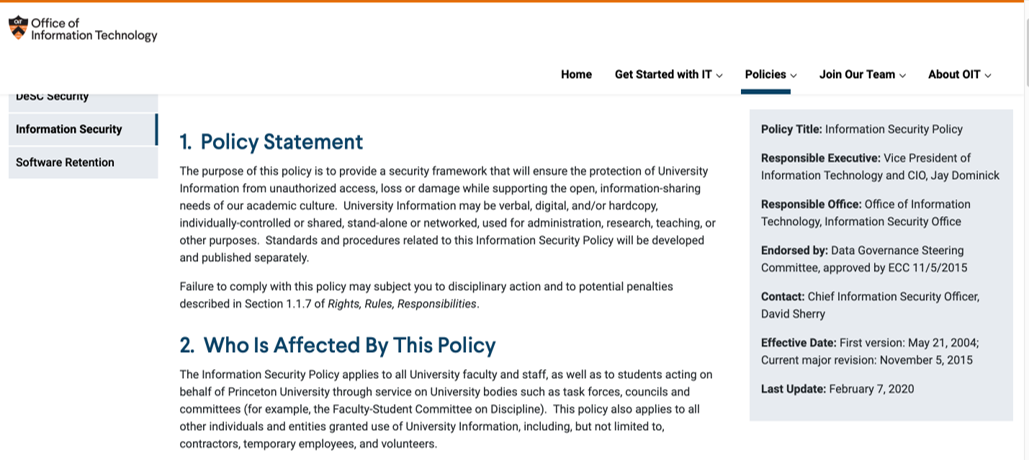
\includegraphics[width=\linewidth]{security_policy_example.png}
\end{figure}

\newpage

\subsubsection{Clause 6; Planning}
The \colorbox{yellow}{organisation shall plan};\\
\bulletPoint Actions to \colorbox{yellow}{address risks and opportunities}\\
\begin{tabular}{r |@{\bulletPoint} l}
   & Define and apply an information security \colorbox{yellow}{risk assessment process} \\
\end{tabular}\\
\bulletPoint How to \colorbox{yellow}{implement the actions} into its ISMS processes\\
\begin{tabular}{r |@{\bulletPoint} l}
   & Define an information security \colorbox{yellow}{risk treatment process} \\
\end{tabular}\\
\bulletPoint How to \colorbox{yellow}{evaluate the effectiveness of these actions}\\
\begin{tabular}{r |@{\bulletPoint} l}
   & Risk monitoring and review \\
\end{tabular}\\

For the controls of risk treatment,\\
The organisation shall;\\
\bulletPoint \colorbox{yellow}{Determine controls} necessary to \colorbox{yellow}{implement} the chosen risk \colorbox{yellow}{treatment options}\\
\begin{tabular}{r |@{\bulletPoint} l}
   & Organisations can design controls as required \\
\end{tabular}\\
\bulletPoint \colorbox{yellow}{Compare the controls} determined in step above with those in ISO/IEC 27002 (Annex A) \\
\begin{tabular}{r |@{\bulletPoint} l}
   & Verify no necessary controls have been omitted \\
\end{tabular}\\
\bulletPoint \colorbox{yellow}{Produce a Statement of Applicability} containing justifications for both inclusions and exclusions of ISO/IEC 27002 controls (Annex A)

For the Security objectives,\\
The organisation shall;\\
\bulletPoint \colorbox{yellow}{Establish information security objectives}:\\
\begin{tabular}{r |@{\bulletPoint} l}
   & \colorbox{yellow}{Consistent} with information security policy                                           \\
   & Be \colorbox{yellow}{measurable} (if practicable)                                                        \\
   & \colorbox{yellow}{Take into account applicable information} security requirements, and results from risk \\& - assessment and risk treatment \\
   & Be \colorbox{yellow}{communicated}                                                                       \\
   & Be \colorbox{yellow}{updated} as appropriate                                                             \\
\end{tabular}\\
\bulletPoint The organisation shall \colorbox{yellow}{retain documentation} on the information security objectives

\subsubsection{Clause 7; Support}
The organisation shall;\\
\bulletPoint (Resources)\\ \colorbox{yellow}{Provide the resources} needed for the ISMS\\
\bulletPoint (Competence)\\ \colorbox{yellow}{Ensure persons have appropriate education}, training, or experience\\
\bulletPoint (Awareness)\\ Ensure persons are \colorbox{yellow}{aware} of the information security policy and the \colorbox{yellow}{implications} of not conforming with the ISMS requirements\\
\bulletPoint (Communication)\\ \colorbox{yellow}{Determine the need for internal and external communications} relevant to the ISMS\\
\bulletPoint (Documentation)\\ Generate required \colorbox{yellow}{documentation}

\newpage

\subsubsection{Clause 8; Operation}
The organisation shall;\\
\bulletPoint \colorbox{yellow}{Plan and control the processes needed to meet security requirements}\\
\bulletPoint \colorbox{yellow}{Perform security risk assessments at planned intervals} or when significant \colorbox{yellow}{changes are} \colorbox{yellow}{proposed or occur}\\
\bulletPoint \colorbox{yellow}{Implement} the information security \colorbox{yellow}{risk treatment plan}\\
\bulletPoint \colorbox{yellow}{Retain documented information} of the results of the information security risk assessment and treatment

\subsubsection{Clause 9; Performance evaluation}
The organisation shall;\\
\bulletPoint \colorbox{yellow}{Evaluate the effectiveness} of the ISMS\\
\bulletPoint \colorbox{yellow}{Conduct internal audits at planned intervals} to check\\
\begin{tabular}{r |@{\bulletPoint} l}
   & ISMS conforms  to the organisation’s own requirements for its ISMS \\
   & and the requirements of ISO/IEC 27001                              \\
\end{tabular}\\
\bulletPoint \colorbox{yellow}{Regularly review} the ISMS to ensure its continuing suitability, adequacy and effectiveness\\
\bulletPoint \colorbox{yellow}{Retain documentation} of all these aspects\\

\subsubsection{Clause 10; Improvement}
\bulletPoint \colorbox{yellow}{When a nonconformity occurs}, organisation shall:\\
\begin{tabular}{r |@{\bulletPoint} l}
   & \colorbox{yellow}{React} to the nonconformity, and, as applicable: \\
\end{tabular}\\
\begin{tabular}{r |@{   \bulletPoint} l}
  |\hspace{\parindent} & Take action to control and correct it \\
  |\hspace{\parindent} & Deal with the consequences            \\
\end{tabular}           \\
\bulletPoint \colorbox{yellow}{Make changes} to the ISMS, if necessary\\
\bulletPoint Shall continually improve the suitability, adequacy and effectiveness of the ISMS

\newpage

\subsection{ISO/IEC 27002}
ISO/IEC 27002 is the \colorbox{yellow}{Code of practice for information security controls}

Provides a \colorbox{yellow}{catalogue} of state of the art security controls

ISO/IEC 27001 requires them \colorbox{pink}{all to be considered} for use as part of an ISMS, and reasons given for excluding any\\
\bulletPoint Statement of Applicability

Contains \colorbox{yellow}{Guidance on security policies} \& List of 34 control objectives\\
\bulletPoint under each control objective, a number of specific controls to achieve the objective\\
\bulletPoint under each control, implementation guidance and other information relevant to that control.

\subsection{ISO/IEC 27006}
It is entitled \colorbox{yellow}{Guidelines for ISMS auditing}

Specifies \colorbox{yellow}{requirements and gives guidance} for bodies providing \colorbox{yellow}{audit} and ISMS certification in accordance with ISO/IEC 27001

Primarily intended to \colorbox{yellow}{support accreditation} of bodies providing ISMS certification according to ISO/IEC 27001

\section{Other Standards}

\subsection{PCI-DSS}
Payment Card Industry (PCI) Data Security Standard\\
\colorbox{yellow}{Addresses cardholder data security}

Provides a \colorbox{pink}{baseline} of technical and operational requirements to \colorbox{yellow}{protect account data}

It \colorbox{pink}{applies to all involved in card processing}\\
\bulletPoint Merchants, processors, acquirers, issuers, and service providers.

Also applies to all other entities that store, process or transmit cardholder data

\newpage

\subsection{Cyber essentials}
\colorbox{yellow}{Government Scheme to improve cyber security of UK companies}\\
Initially started as a best practice document\\
Now it offers two different schemes\\
\bulletPoint Cyber Essentials\\
\bulletPoint Cyber Essentials Plus

Self-assessment of 5 \colorbox{cyan}{Practices/technical controls}\\
\bulletPoint Secure your \colorbox{yellow}{Internet} connection\\
\bulletPoint Secure your \colorbox{yellow}{devices} and software\\
\bulletPoint Control access to your \colorbox{yellow}{data and services}\\
\bulletPoint Protect from viruses and other \colorbox{yellow}{malware}\\
\bulletPoint Keep your devices and \colorbox{yellow}{software up to date}\\
Cyber Essentials \colorbox{green}{Plus}\\
\bulletPoint An \colorbox{yellow}{external assessor} conducts an audit to test the same five controls

\chapter{Guest lecture - Data Protection}

\begin{center}
  \begin{Large}
    \textbf{
      \color{white}
      \colorbox{red}{THIS CHAPTER IS NOT EXAMINABLE}}
  \end{Large}
\end{center}

UK GDPR post Brexit the \colorbox{pink}{GDPR was retained in domestic law}, but the UK has the
independence to keep the framework under review  with the potential to diverge
from EU standards

GDPR definition: \colorbox{green}{personal data} means any \colorbox{yellow}{information relating} to an
identified or \colorbox{yellow}{identifiable} \colorbox{yellow}{natural person} (‘data subject’)\\
e.g., name, address, salary, photograph, IP address, email, etc.

\colorbox{green}{Special category data};\\
Formerly known as sensitive personal data, this data can \colorbox{yellow}{only be processed in certain circumstances}.\\
Special category data covers the following:\\
\bulletPoint Racial/ ethnic origin\\
\bulletPoint Political opinions\\
\bulletPoint Religious or philosophical beliefs\\
\bulletPoint Membership of a Trade Union\\
\bulletPoint Health data\\
\bulletPoint Sexual orientation/ sex life\\
\bulletPoint Genetic data (primarily relating to DNA)\\
\bulletPoint Biometric data (examples include facial recognition, iris scanning, fingerprint scanning, voice recognition)

The GDPR defines \colorbox{green}{processing} as:\\
\colorbox{yellow}{any operation} or set of operations which is \colorbox{yellow}{performed on personal data} or on
sets of personal data, whether or not by automated means, such as collection,
recording, organisation, structuring, storage, adaptation or alteration,
retrieval, consultation, use, disclosure by transmission, dissemination or
otherwise making available, alignment or combination, restriction, erasure
or destruction.

Lawful basis for processing personal data;\\
\bulletPoint Consent:\\
Data subject gives clear, specific, and freely given consent.\\
\bulletPoint Contractual Necessity:\\
Processing is necessary for the performance of a contract.\\
\bulletPoint Legal Obligation:\\
Processing is required to comply with a legal obligation.\\
\bulletPoint Vital Interests:\\
Processing protects the vital interests of the data subject.\\
\bulletPoint Legitimate Interests:\\
Processing is necessary for legitimate interests, not overridden by the data subject's rights and interests.\\
\bulletPoint Public Task:\\
Processing is necessary for the performance of an official task carried out in the public interest or in the exercise of official authority.

\newpage

Lawful basis for special category data;\\
\bulletPoint  Consent:\\
Explicit and informed permission from the data subject.\\
\bulletPoint Contractual Necessity:\\
Processing necessary for contract performance.\\
\bulletPoint Legal Obligation:\\
Compliance with legal requirements.\\
\bulletPoint Vital Interests:\\
Protecting life or health when consent is impossible.\\
\bulletPoint Employment:\\
Obligations related to employment law.\\
\bulletPoint Public Interest:\\
Reasons of substantial public interest.\\
\bulletPoint Health and Social Care:\\
Medical and social care purposes.\\
\bulletPoint Public Health:\\
Safeguarding public health interests. (e.g. COVID-19)\\
\bulletPoint Research:\\
Archiving, scientific, or historical research in the public interest\\
\bulletPoint Legal Claims:\\
For legal claims and judicial acts.\\

\colorbox{cyan}{Principles} of Data Protection;\\
\bulletPoint Lawfulness, Fairness, and Transparency:\\
Personal data must be processed lawfully, fairly, and transparently.\\
\bulletPoint Purpose Limitation:\\
Data should be collected for specific, explicit, and legitimate purposes.\\
\bulletPoint Data Minimisation:\\
Only the necessary data should be collected and processed for the intended purpose.\\
\bulletPoint Accuracy:\\
Data must be accurate and kept up to date where necessary.\\
\bulletPoint Storage Limitation (retention)\\
Data should be kept for no longer than is necessary for the intended purpose.\\
\bulletPoint Integrity and Confidentiality (security):\\
Data must be processed securely and protected against unauthorised access or disclosure.\\
\bulletPoint Accountability and Governance:\\
Organisations are responsible for complying with the principles and demonstrating compliance.

\colorbox{cyan}{Data Subject Rights};\\
\bulletPoint Right to Access:\\
Data subjects can request access to their personal data held by Royal Holloway \\
\bulletPoint Right to Rectification:\\
Data subjects can request the correction of inaccurate or incomplete data.\\
\bulletPoint Right to Erasure (Right to Be Forgotten):\\
Data subjects can request the deletion of their data under certain conditions. This is not an absolute right\\
\bulletPoint Right to Restrict \\
Processing: Data subjects can request the temporary restriction of their data processing.\\
\bulletPoint Right to Data Portability:\\
Data subjects can request their data in a commonly used, machine-readable format.\\
\bulletPoint Right to Object:\\
Data subjects can object to their data processing for specific reasons.

\newpage

Subject Access Requests (\colorbox{green}{SARS}) \\
There is a direct link if a workplace invests in employees' satisfaction and
transparency, as it significantly reduces the likelihood of employees filing
SARs or complaints. \\
Increase staff awareness of data discovery with SARs.

\colorbox{green}{Police Requests} + Other Agencies Requests\\
When the police or other law enforcement authorities requires access to personal
data, it is crucial to understand that such a request does not automatically
grant them the right to obtain this information. \\
If a police request is received by the University, it is important to ensure
that the request is accompanied by Data Protection Agreement (\colorbox{pink}{DPA}) form to
ensure that any disclosure of personal data is lawful. \\
The University also receives requests from the Home Office, Councils, NHS.

\colorbox{green}{Erasure Requests}  \\
IT and DP continue to work together to improve the processing of Erasure requests. \\
When the University receives an Erasure request, it is crucial to evaluate the
request in light of the Retention Policy. A \colorbox{green}{Retention Policy} determines how long
different types of data should be retained and when it can be disposed of. \\
AI and data dispersement is an ongoing challenge.

\section{Data Breaches}

Definition  ‘a \colorbox{green}{breach} of security leading to the \colorbox{yellow}{accidental or unlawful}
destruction, loss, alteration, unauthorised disclosure of, or access to,
\colorbox{yellow}{personal data} transmitted, stored or otherwise \colorbox{yellow}{processed};’\\
(Depending on severity are reportable to ICO)

\colorbox{green}{Non-material damage} - This covers psychological harm and distress caused by the breach, including:\\
Anxiety and stress, Loss of sleep, Feelings of vulnerability or violation of privacy

\colorbox{green}{Material damage} - This refers to financial losses or costs incurred as a result of the breach, such as:\\
Identity theft leading to financial fraud, Costs of credit monitoring services, Expenses related to mitigating the effects of the breach

\newpage

\subsection{Prevention}

A good guideline is to refrain from documenting anything you wouldn't feel comfortable saying directly to the person. Remember, a requester has the right to access all emails related to them.

Where appropriate please mark emails Confidential

Password protect sensitive attachments.  Use Teams Groups to limit access and circulation

The ICO can, in the event of non-compliance with the legislation, issue the following:\\
\bulletPoint An information notice – require information for an investigation\\
\bulletPoint An assessment notice – require an organisation to permit the Commissioner to carry out an assessment of whether the organisation has complied or is complying with the data protection legislation\\
\bulletPoint An enforcement notice – requirement to start or stop certain activities which have resulted in a breach of the legislation\\
\bulletPoint A penalty notice – where a failing is sufficient, or one of the notices above has not been complied with, the ICO can issue a fine of up to €10m or 2\% of annual turnover or, in more severe cases, a fine of up to €20m or 4\% of annual turnover

\section{Threats}

\begin{figure}[H]
  \centering
  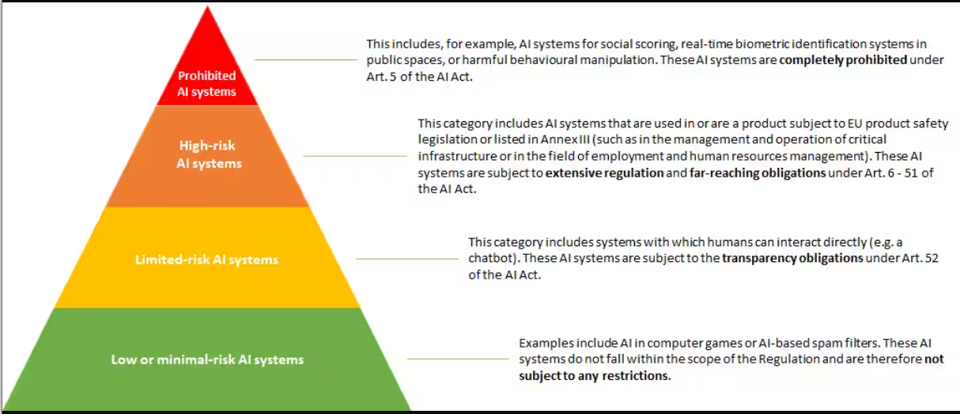
\includegraphics[width=\linewidth]{EU AI act risk assessment.png}
  \caption{EU AI act risk assessment}
\end{figure}

Privacy Enhancing Technologies (\colorbox{green}{PET});\\
\colorbox{yellow}{Tools and techniques that protect privacy while enabling data analysis}\\

Examples;\\
Homomorphic Encryption,
Differential Privacy,
Federated Learning,
Anonymisation,
Secure Multi-Party Computation

Purpose: Minimise personal data use, Maximise data security, Empower individuals\\
Benefits: Enhanced data protection, Regulatory compliance, Valuable insights while preserving privacy

\chapter{Unit 3 - Risk}

Risk assessments can make you think negatively \\
Risk assessment can make you think small

\section{Risk Culture}

\colorbox{pink}{Risk is good}; Businesses take risks in order to make money\\
The \colorbox{pink}{hard part is accurately assessing risk} \\
The team that balances risk most effectively survives

Risk Domains\\
Finance;\\
\bulletPoint Exact \\
\bulletPoint Known \\
\bulletPoint Visible\\
\bulletPoint Occasional ‘Black Swans’ hit whole economy\\
Cyber;\\
\bulletPoint Vague \\
\bulletPoint Unknown \\
\bulletPoint Sudden\\
\bulletPoint Failure is lonely

Need to check if an Organization's risk culture \colorbox{pink}{appropriate} for the sector\\
Do people take a well judged approach to risk for their role

Larger companies generally are more risk averse.  \\
Smaller companies become larger companies by being risk-friendly;
“let’s do it and be legends”

\colorbox{green}{Risk culture} is a \colorbox{yellow}{set of norms}, attitudes
and behaviours \colorbox{yellow}{related to} awareness, management and controls of \colorbox{yellow}{risks}

\section{Doing Risk Assessments well}

\colorbox{green}{Risk} definitions;\\
- Probability of something harmful to happen\\
- ISO/IEC 31000; \colorbox{yellow}{Effect of uncertainty on objectives}\\
- ISO/IEC 27005; Potential that a given threat will exploit vulnerabilities of
an asset or group of assets and thereby cause harm to the organization

\subsection{Listing risks}

All methods for listing risks boil down giving you a list of risks and asking
you if any of them apply to your situation

\subsubsection{Joe's Way}

Step 1: \colorbox{yellow}{Write down everything that you are worried about}.\\
Put an asterisk by them because you don’t have a clear view on them.\\
\colorbox{pink}{Someone else} should do the likelihood and impact of those

Step 2: \colorbox{yellow}{Work through your (approved) ‘trigger list’};\\
\bulletPoint your list of assets \\
\bulletPoint your list of laws (or court cases) \\
\bulletPoint your list of stakeholders \\
\bulletPoint Software components \\
\bulletPoint your future plans.\\
\bulletPoint your list of attackers\\
Then look at \colorbox{yellow}{combinations} (each asset with each law with each stakeholder)

\subsubsection{Microsoft's Way - STRIDE}

Spoofing \\
Tampering\\
Repudiation\\
Information Disclosure \\
Denial of service\\
Elevation of privilege

Consider how \colorbox{yellow}{each threat category could impact} the component and what \colorbox{yellow}{vulnerabilities might} \colorbox{yellow}{be exploited}.

\subsubsection{Versprite’s Way}

PASTA! - The Process of Attack Simulation and Threat Analysis!\\
Seven stages – includes listing attack surfaces, decomposing the model. That sort of thing.

\subsection{Risk Likelihood}

\colorbox{yellow}{Subjective}: Impossible, Possible, Unlikely, Likely, definite\\
“I feel good about this ”

\colorbox{yellow}{Objective}: 1,2,3,4,5\\
“This happened four times to us last year and six times to our competitor”\\
“This will either happen to us or Pepsi depending on X” \\
“The accountant thinks it’s 50-50”

Even if the rating is incorrect the act of rating is a powerful \colorbox{pink}{way of focusing attention} on the risk

\colorbox{pink}{Humans are terrible at risk}. \\
We understand 50-50 well, and pretty good at 99-1 but terrible at 60-40.  \\
We also rate things as more likely if they are dramatic (plane crashes compared to long-illness)\\
Also unprovable – people win lotteries.

\subsubsection{Risk by Microsoft - DREAD}

Damage\\
Reproducibility\\
Exploitability\\
Affected Users\\
Discoverability \\
Detection

DREAD does \colorbox{yellow}{both likelihood and impact} (judge and jury) \\
Seen as \colorbox{pink}{problematic} these days and quietly removed.

\subsubsection{Risk by YOUR COMPANY}

\colorbox{yellow}{Have stakeholders do it} and average it -  Include your line manager\\
Develop your \colorbox{yellow}{own formula} that \colorbox{pink}{keeps everybody happy}.

\subsection{IMPACT}

\colorbox{pink}{Same subjective/objective problem} as before, but now you can use money or another central \colorbox{yellow}{proxy} (“lives saved”).

\colorbox{yellow}{Subcategorise} risks according to impact.\\
“This has a 20\% chance of  costing ten grand and a 80\% chance of costing half a million”

You can ask the question “how many of these have to go wrong before we go bankrupt/lose our jobs?”

\colorbox{yellow}{Convert your impact proxy} into a single digit. \\
Develop a process for conversion at the company if necessary

\begin{figure}[H]
  \centering
  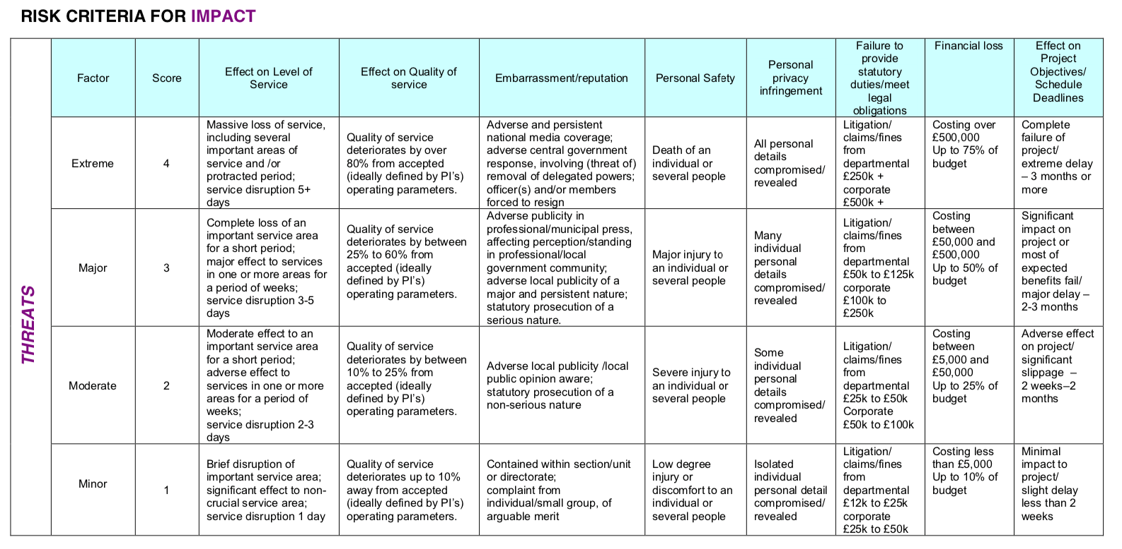
\includegraphics[width=.8\linewidth]{risk impact.png}
  \caption{Royal Borough Windsor and Maidenhead approach to management of Risk}
\end{figure}

\newpage

\subsection{Risk treatment options}
For each risk \colorbox{yellow}{choose one of}: \\
\bulletPoint TRANSFER\\
\bulletPoint TOLERATE \\
\bulletPoint TREAT\\
\bulletPoint TERMINATE

Risk treatment options should be selected \colorbox{yellow}{based on}\\
\bulletPoint Risk assessment itself\\
\bulletPoint Expected cost for implementing options

There are \colorbox{pink}{tools}, hundreds of them. They are very reassuring.\\
Managers like them  Auditors like them \\
They are nice and quantifiable\\
They deal with a \colorbox{pink}{very very narrow} set of possible threats.

\subsubsection{TRANSFER}

Examples;\\
\bulletPoint Insurance \\
\bulletPoint Third party suppliers (to ‘take the blame’ not ‘solve the problem’)  \\
\bulletPoint Banks/invoice markets \\
\bulletPoint Project Partners

\subsubsection{TOLERATE}

\colorbox{pink}{Sometimes} ignoring the issue is the right decision. But not often

This is a valid approach when the risk level is very low, or when mitigation
is extremely expensive (for example: product recalls)

\subsubsection{TREAT}

\colorbox{yellow}{Do something about the risk}\\
\bulletPoint Reduce Likelihood (as cheaply as possible)  \\
\bulletPoint Reduce Impact (as cheaply as possible) \\
\bulletPoint Reduce Both! \\
\bulletPoint Consider second-order risks.

\subsubsection{TERMINATE}

“Nope”\\
\colorbox{pink}{Only useful for certain risks}. You can’t terminate having customers, but you
could terminate a risky expansion in a new country.

Can be recognising a structural problem “we don’t need that group/paperwork/process any more” \\
check for second order effects

\subsection{Communication}

Risks and their treatment \colorbox{yellow}{must be communicated} to managers and operational staff

\colorbox{yellow}{Even before risk treatment}, information about identified risks can be \colorbox{pink}{very
  valuable} to manage incidents and may reduce damage.

It’s good practice generally for everybody to know what the organisation cares about.

\subsection{Alternative approach}

Compliance - \colorbox{yellow}{Just stick to the rules!}

\section{Is it a good risk assessment?}

A risk assessment is \colorbox{yellow}{can only be judged against a particular situation}\\
Like a map can only be judged against the thing it’s a map of.

A risk assessment, like all strategy documents gets its power from the buy in and the communication. \\
“Every time we run out of X in the warehouse we loose £10k a day, so I’m going to be getting that right”

\chapter{Unit 4 - Security Controls}

There are \colorbox{cyan}{two ways of viewing controls}; The risk way and the algorithm way

The \colorbox{green}{risk view} of controls;\\
\bulletPoint Your \colorbox{yellow}{risk assessment} is a \colorbox{yellow}{list of risks to the security objectives}.\\
\bulletPoint Every \colorbox{yellow}{risk could be linked} to a security objective\\
\bulletPoint Every risk will \colorbox{yellow}{need to be controlled}.\\
\bulletPoint The things that \colorbox{yellow}{control risks} are called \colorbox{green}{‘controls’}

The \colorbox{green}{algorithm view} of controls;\\
\bulletPoint \colorbox{yellow}{Companies} exist as \colorbox{yellow}{algorithms} for making \colorbox{yellow}{the most money possible}. \\
\bulletPoint \colorbox{yellow}{Some are more effective} algorithms than others. \\
\bulletPoint \colorbox{yellow}{Most programming styles} can be \colorbox{yellow}{seen in business}:  procedural, logic, constraint. \\
\bulletPoint \colorbox{yellow}{Some} languages \colorbox{yellow}{deliberately designed for business}: Cobol, B method.\\
\bulletPoint \colorbox{yellow}{Designing} these algorithms is \colorbox{yellow}{hard} (and well paid)

This (IY3501) is a course on ‘how to design the security part of  the business algorithm’

\colorbox{yellow}{ISO 27001} is a standard for \colorbox{yellow}{‘is the security part of the business algorithm doing what is} \colorbox{yellow}{normally expected?’}

Controls are the way you build the security part of the business algorithm.

A security \colorbox{green}{control} is \colorbox{yellow}{a measure that modifies risk}.

Security controls include:\\
\bulletPoint Security policies\\
\bulletPoint Processes\\
\bulletPoint Devices and technology\\
\bulletPoint Practices

Controls are \colorbox{pink}{a governance-level term}. \\
Typically applied as financial controls: budgets; multiple signatories; cash flow; debt management \\
But a company might have environmental controls; HR controls; IT controls and Operational controls.\\
Colloquially used the same as ‘policy’

The \colorbox{cyan}{third view};\\
Controls are the (often literal) \colorbox{yellow}{cost of achieving the security objectives}.

\section{ISO/IEC 27002}

The \colorbox{yellow}{catalogue} of state of the art security controls

\newpage

Four \colorbox{cyan}{categories} of controls (TOPP):\\
\bulletPoint Technological\\
\bulletPoint Organizational \\
\bulletPoint People \\
\bulletPoint Physical

Each category contains between 8 (People) and 37 (Organizational) controls

The controls are \colorbox{cyan}{divided} as\\
people, if they concern individual people;\\
physical, if they concern physical objects;\\
technological, if they concern technology;\\
otherwise they are categorized as organizational.

Each control has some attributes\\
\colorbox{green}{Operational capabilities} are \colorbox{green}{Security Domains} - \colorbox{yellow}{different groupings of the same controls}

\subsection{Organisational Controls}

5.3 Segregation of duties \\
5.7 Threat intelligence\\
5.11 Return of assets \\
5.32 Intellectual property rights\\
(several of the controls in this category are about incidence response)

\begin{figure}[H]
  \centering
  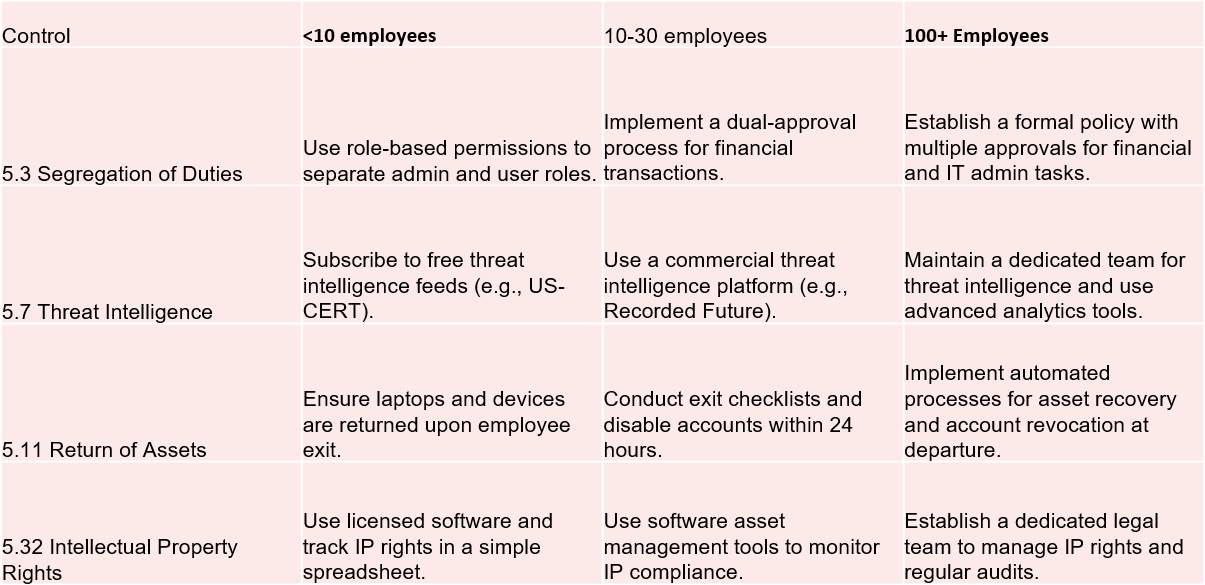
\includegraphics[width=\linewidth]{organizational controls.png}
\end{figure}

\subsection{Physical Controls}

7.7 Clear desk and clear screen \\
7.10 Storage Media\\
7.12 Cabling security\\
7.13 Equipment maintenance

\subsection{People Controls}

Will be covered later\\
- a project manager leaving is a code smell

\subsection{Technical Controls}

8.15 Logging\\
Contrast with ‘no blame culture’\\
8.17 Clock synchronization\\
8.25 Secure Development life cycle.\\
8.31 Separation of development, test and production environments \\
8.43 Protection of information systems during audit testing.

\begin{figure}[H]
  \centering
  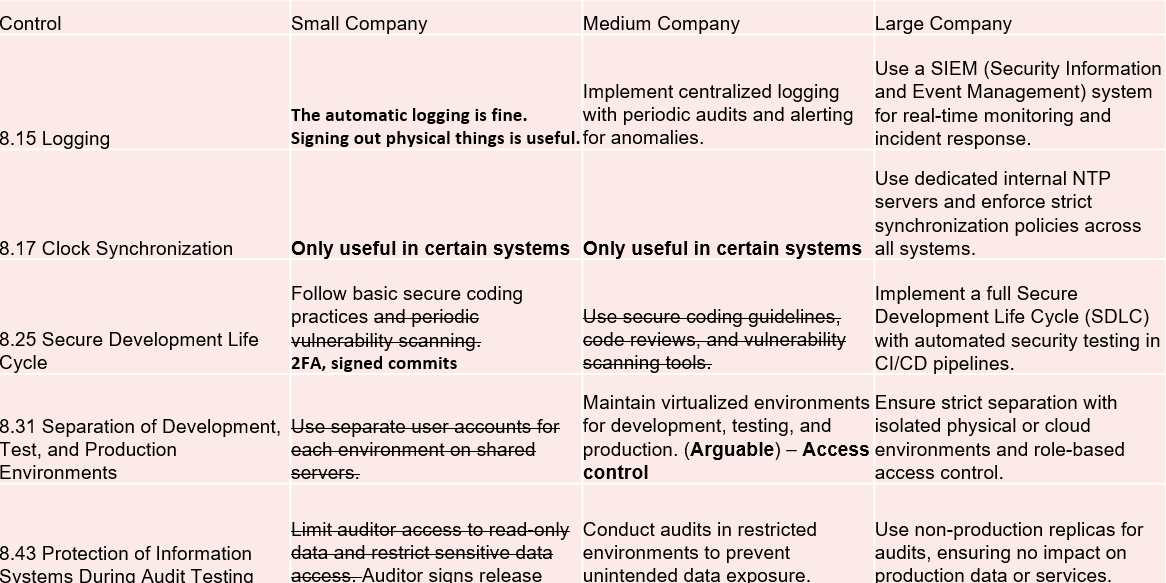
\includegraphics[width=\linewidth]{technical controls.png}
\end{figure}

\section{Security policies}

\colorbox{yellow}{Clause 5} - Leadership \colorbox{yellow}{required a policy}

A \colorbox{green}{security policy} is
\colorbox{yellow}{intentions and direction of an organization as formally expressed by its} \colorbox{yellow}{top management}.

In an \colorbox{yellow}{ISMS}, a security policy \colorbox{yellow}{provides the framework} for \colorbox{yellow}{setting} information security \colorbox{yellow}{objectives}

Security policies \colorbox{pink}{depend on the organisational unit}\\
\bulletPoint High-level security policies defined by senior management\\
\bulletPoint Low-level security policies for specific units/processes

\colorbox{yellow}{A security policy is a kind of control}

Goal;\\
To provide management direction and support for information security in
accordance with business requirements and relevant laws and regulations

Two \colorbox{cyan}{levels};\\
\bulletPoint High-level: 1 global policy\\
\bulletPoint Low-level: n topic-specific policies

\subsection{Top-Level Security Policy}

\colorbox{yellow}{Defined and approved by top management}\\
\colorbox{yellow}{Outlines} the organisation’s \colorbox{yellow}{approach} to information security\\
Should be \colorbox{Salmon}{published and communicated} to all employees and relevant parties

Should include\\
\bulletPoint \colorbox{yellow}{definition} of information security, \colorbox{yellow}{objectives and principles} to guide all activities relating to information security\\
\bulletPoint assignment of general and specific \colorbox{yellow}{responsibilities} for ISM to defined roles\\
\bulletPoint \colorbox{yellow}{processes} for handling deviations and exceptions

\subsection{Low-level Policies}

Top-level specific policy \colorbox{pink}{must be supported} by low-level, topic-specific policies\\
These cover \colorbox{yellow}{implementation} of information security controls

E.g.,\\
\bulletPoint Backup\\
\bulletPoint Information transfer\\
\bulletPoint Protection from malware\\
\bulletPoint Management of technical vulnerabilities\\
\bulletPoint Cryptographic controls\\
\bulletPoint Communications security\\
\bulletPoint Privacy and protection of personally identifiable information \\
\bulletPoint Access control \\
\bulletPoint Information classification (and handling)\\
\bulletPoint Physical and environmental security \\
End user oriented topics;\\
\bulletPoint acceptable use of assets\\
\bulletPoint clear desk and clear screen\\
\bulletPoint information transfer\\
\bulletPoint mobile devices and teleworking\\
\bulletPoint restrictions on software installations and use

The \colorbox{pink}{need} for internal policies for information security \colorbox{pink}{varies}\\
Especially useful in larger and more complex organisations, where those defining the levels of control are separated from those implementing the controls

Policies can be issued in a single or as a set of related documents

\subsection{Communication}

Policies should be \colorbox{yellow}{communicated} to employees and relevant external parties in a form that is \colorbox{yellow}{relevant, accessible and understandable} to the intended reader

How?\\
\bulletPoint Training and awareness\\
\bulletPoint Mailing campaigns\\
\bulletPoint Posters around the building\\
\bulletPoint Other?

\subsection{Reviews}

Security policies should be \colorbox{yellow}{reviewed at planned intervals}, or whenever \colorbox{yellow}{significant changes} \colorbox{yellow}{occur}, to \colorbox{pink}{ensure their continuing adequacy}

Each policy \colorbox{yellow}{should have an owner}, responsible for its development\\
Review should include assessing opportunities for \colorbox{yellow}{improvement} of policies

\chapter{Unit 5 - Incident Management and Disaster Recovery}

Security events and incidents \colorbox{pink}{will happen}\\
\colorbox{yellow}{Planning} for them will (hopefully) \colorbox{yellow}{reduce the impact} of them \colorbox{pink}{on the business objectives}

\colorbox{cyan}{Plans} include\\
\bulletPoint Incident response\\
\bulletPoint Business continuity\\
\bulletPoint Disaster recovery

\section{Introduction to Incident Management}

\colorbox{yellow}{The best defence is a good offence}\\
In business terms this might be ‘make so much money that you can buy protection/your way out of incidents’

Information security \colorbox{green}{incident management} is a \colorbox{yellow}{set of ‘processes} for detecting,
reporting, assessing, responding to, dealing with, and learning from information security \colorbox{yellow}{incidents}’.
(ISO 27000)

A Information Security \colorbox{green}{Event} is an \colorbox{yellow}{‘identified occurrence} of a system, service
or network \colorbox{yellow}{state indicating a possible breach of} information security \colorbox{yellow}{policy}
\colorbox{yellow}{or failure of controls, or} a previously \colorbox{yellow}{unknown situation} that may be
\colorbox{yellow}{security relevant}’ (ISO 27000)

A Information Security \colorbox{green}{Incident} is a \colorbox{yellow}{‘single or a series of unwanted or
  unexpected} information security \colorbox{yellow}{events} that have a \colorbox{yellow}{significant probability} of
\colorbox{yellow}{compromising business operations} and \colorbox{yellow}{threatening} information \colorbox{yellow}{security}’.
(ISO 27000)

Event: something you make a note of.\\
Incident: something you actively do something about.\\
Security incidents are \colorbox{Salmon}{instantiated risks}

E.g.,\\
\bulletPoint Wireless network down\\
Event (from a security perspective; it’s an incident for the IT team) – also ‘It depends’ \\
\bulletPoint Customer private data available publicly\\
Incident and event\\
\bulletPoint Anti-virus alert\\
Event\\
\bulletPoint Computer infected by ransomware\\
Incident

\newpage

No matter how carefully an organisation conducts its business, and regardless of the security controls,
Security incidents will happen

Security \colorbox{pink}{events can affect} confidentiality, integrity and/or availability of assets\\
It is therefore important to have plans in place to deal with security events before they occur\\
Trying to \colorbox{pink}{implement solutions afterwards is likely to be ineffective}

Top priority is to \colorbox{yellow}{ensure everyone knows}
how to \colorbox{yellow}{recognise} an incident, and who to \colorbox{yellow}{report} it to\\
Can be achieved in a variety of ways

How closely to follow the plan will be an operational decision at the time. \\
“No plan survives contact with the enemy”

But ‘not following the plan’ can lose you your job\\
What is the \colorbox{pink}{authority of ‘the plan’?} Can the CEO override it?  The COO?

\subsection{Managing an incident}

Five \colorbox{cyan}{phases}: \\
\bulletPoint Reporting\\
\bulletPoint Investigation\\
\bulletPoint Assessment\\
\bulletPoint Corrective actions\\
\bulletPoint Review

\colorbox{cyan}{Separate} out the five phases \colorbox{yellow}{by communication} \\
\bulletPoint Reporting: “Boss, this happened” \\
\bulletPoint Investigation “Boss, we think this is why it happened”\\
\bulletPoint Assessment “Boss, X,Y and Z are going to happen, we think we should do ABC” \\
\bulletPoint Corrective actions “Boss, it’s handled” \\
\bulletPoint Review “Boss, we’re still checking that thing” \\
This keeps the phases from merging and forces documentation.


\subsubsection{Phase 1: Reporting}

Good practice to have an incident \colorbox{yellow}{report form}\\
\bulletPoint Identity of event reporter with contact, location and dept.\\
\bulletPoint Brief description of incident\\
\bulletPoint Whether there is danger to life, heath or assets\\
\bulletPoint Other potential impact to business operations\\
\bulletPoint Description of any actions taken in response\\
\bulletPoint Time incident first noticed\\
\colorbox{yellow}{All actions taken after report should be logged}

Logging - \colorbox{yellow}{Contemporaneous} (or ‘live’) notes. \\
can be Photos, screenshots \\
Use messaging software where possible rather than phone calls.

Think about two \colorbox{cyan}{sets of notes}: \\
\bulletPoint One to protect the company.\\
\bulletPoint One to protect you from the company\\
Make sure the logs aren’t \colorbox{pink}{data-breaches on their own}.

Examples of Reporting:\\
\bulletPoint Bug report \\
\bulletPoint Child Protection disclosure \\
\bulletPoint Alert from ISMS framework

\subsubsection{Phase 2: Investigation}

Set of \colorbox{cyan}{actions taken} to identify\\
\bulletPoint Origin of the incident\\
\bulletPoint Impact to business\\
\bulletPoint Security failures that led to the incident\\
\bulletPoint Law and regulatory implications\\
\colorbox{yellow}{Investigation} makes use of logs, interviews, etc

Investigation should not destroy evidence - \colorbox{yellow}{maintain a chain of custody}


\subsubsection{Phase 3: Assessment}

Very similar to \colorbox{yellow}{risk assessment}, except this time it’s real\\
All the principles about careful consideration apply

Identify potential impact of the incident - How it will affect the business operation\\
\colorbox{pink}{Prioritise} assets that may be more relevant for business operation


\subsubsection{Phase 4: Corrective actions}

Similar to risk \colorbox{yellow}{treatment options}

\colorbox{yellow}{Apply} a set of actions that correct or mitigate the incident\\
All actions should be logged into the incident report form

Actions need to be \colorbox{pink}{proportionate} and according to the \colorbox{pink}{urgency} of the incident

\subsubsection{Phase 5: Review}

The incident should be \colorbox{yellow}{monitored} to ensure that corrective actions are \colorbox{yellow}{working as intended}\\
If not, a new process may be started

Very similar to other review security management processes\\
Make sure to set up an event for proper ‘learning’

\subsubsection{Learning from Security Incidents}

\colorbox{yellow}{Knowledge gained} from analysing and resolving information security incidents should
be used to \colorbox{yellow}{reduce the likelihood or impact of future incidents}

Mechanisms should be in place to \colorbox{yellow}{help quantify and monitor} the types, volumes
and costs of information security incidents

Information gained from evaluating security incidents should be used to \colorbox{yellow}{identify recurring} or \colorbox{yellow}{high impact} incidents

\subsubsection{Incident response teams (IRT)}
\colorbox{yellow}{Employees in charge of responding to incidents}

IRT members need to come \colorbox{yellow}{from across the organisation} so there is \colorbox{pink}{breadth of knowledge} to \colorbox{pink}{deal effectively} with incidents of all types\\
Should also be \colorbox{yellow}{senior and experienced} so they have \colorbox{pink}{authority to make quick decisions}

They should be able to \colorbox{pink}{call on additional resources} (internal or external) as needed

There needs to be a \colorbox{yellow}{documented escalation process} for the IRT to reach senior members of the organisation if necessary

Each IRT team member should have a copy of the incident response plan documentation, and \colorbox{pink}{should always be readily contactable}

\subsubsection{Incident response procedures}

Incident management procedures should be \colorbox{yellow}{broad in scope}\\
It is \colorbox{pink}{difficult to predict} what the \colorbox{pink}{nature of an incident} will be

Some idea of likely events can be obtained from looking at the list of risks from the risk assessment to identify high probability and high impact events\\
Some events, e.g. terrorist activity or freak storm damage, are not part of the normal threat profile

If there is a likelihood of a criminal activity, appropriate authorities should be notified\\
This means it is \colorbox{pink}{vital to understand the legal requirements} for reporting events - keeping evidence secure

In UK it is mandatory to inform police if\\
\bulletPoint There is a suspicion of terrorist activity\\
\bulletPoint Child pornography has been viewed or processed\\
\bulletPoint There are suspicious financial activities

It is important to remember that adopting all the controls given in ISO/IEC 27002
is not mandatory to achieve ISO/IEC 27001 certification.\\
It is simply \colorbox{yellow}{necessary to consider all} of them as part of the organisation’s risk
assessment, and, if they are deemed inappropriate or unnecessary, then it is
fine not to adopt them as long as the reasoning is documented.

\newpage
\section{Disaster Recovery and Business Continuity}

\colorbox{green}{Business continuity};\\
General term used to describe \colorbox{yellow}{measures implemented} by an organisation to enable
it to \colorbox{yellow}{\textbf{continue operating} after a major incident/disaster}

For example\\
\bulletPoint An organisation may have a contract with a service provider to enable access to
a fully equipped office at very short notice, e.g. for recovery after a major fire\\
\bulletPoint Backup can be thought of as part of business continuity planning

A \colorbox{green}{Business Continuity Plan} (BCP) is about \colorbox{yellow}{maintaining continuity} of a business\\
Again, problems will occur, no matter how well run things are, and problems affect
operations

Problems will \colorbox{pink}{vary in seriousness}; A printer out of toner to a power failure

Whatever occurs, the \colorbox{pink}{situation will be better if tried and tested plans are in
  place} to deal with the problem

Business \colorbox{yellow}{continuity fails when the business is no longer operating} (‘continuing’)

Then it’s \colorbox{green}{disaster recovery}\\
Sometimes a problem is so major that \colorbox{yellow}{normal operations are damaged or disrupted
  beyond} \colorbox{yellow}{reasonable or rapid repair}

This is when Disaster Recovery (DR) is required, and \colorbox{yellow}{plans} for dealing with
the most serous problems are a key part of ISM

Key to planning DR is \colorbox{yellow}{risk assessment}\\
some disasters may be so unlikely or so catastrophic that they are not worth
planning for

Sometimes the best choice is to shut down for a day rather than be at 50\% for week.\\
Sometimes that’s the worst possible idea.\\
You have to make a considered choice and hope you made the right one.
\newpage
\subsection{Documentation}

A key \colorbox{yellow}{difference between BC and DR is the scale} of the steps involved\\
\bulletPoint If the plan calls for minor adjustment to normal working practices or to
normal operations, then this should form part of the BCP\\
\bulletPoint DR, by contrast, addresses problems with a wider impact, and
is generally focussed on contingency planning for IT systems

\colorbox{pink}{There will be cyber security focused plans}:\\
Backup data centres, smooth failures, backup services, redundancies.

There also \colorbox{yellow}{needs to be a cyber security view on general plans}:\\
Lots of the possible BC/DR solutions will have serious cyber security implications

A sudden BC change might need you to \colorbox{pink}{rewrite/suspend half the policies you wrote} for cyber security\\
It can then be extremely hard to get people to follow remaining policies when
you’ve suspended a bunch of them.

Different organisations will have \colorbox{pink}{very different needs} for BCPs and DR plans\\
\bulletPoint If only major risk to continued operation of an organisation is loss of key services (e.g. water, electricity, network connectivity),
it may be appropriate simply to ensure that all records are backed-up offsite, without a complex DR plan\\
\bulletPoint In an organisation driven by rapid cash turnover short-term loss of a website could mean a major financial loss

It is \colorbox{pink}{not clear how large} the \colorbox{pink}{scope} of DR plans should be\\
Some organisations have been caught out in the past by not going far enough

For example;\\
When the World Trade Center was attacked in 1993 with bombs in an underground
car park, more than half the companies in the building at the time never
traded effectively again\\
It was months before building was declared safe:  companies lost access to vital records

\colorbox{pink}{Lack of access} is a major issue, \colorbox{pink}{often overlooked}\\
It can be caused by a problem occurring outside the organisation’s premises\\
\bulletPoint For example, in the event of a security threat in a city, a cordon
might be set up denying access to all buildings in a wide area

\colorbox{yellow}{Write your plan for a set of ‘worst case’ scenarios} rather than risk assessment ones

COVID-19 (obviously) caused lots of changes in the world.\\
\bulletPoint In business, all companies were in some version of business continuity/disaster recovery \\
\bulletPoint Because that event is in recent memory, most companies are currently sensible about some types of BC/DR. \\
\bulletPoint However, the processes will soon solidify again (and arguably has)

Many produced a dedicated plan for Covid-19's impacts;\\
\colorbox{yellow}{The better your documentation/communication is in general, the less you need a dedicated} \colorbox{yellow}{disaster plan.}

Documentation of plans is clearly vital; \colorbox{yellow}{Documents need to be available} when needed!\\
Having them in the office, if loss of access to the office is one of the events
covered in the plans, does not make sense

\colorbox{yellow}{Plans need to be available} but they may also need to be \colorbox{yellow}{kept secure}\\
They may contain very sensitive information

\subsection{Outsourcing}

\colorbox{yellow}{Contracts} for the \colorbox{yellow}{provision} of a DR facility are \colorbox{pink}{now common}\\
This changed significantly (worse) during the pandemic

Companies offer standardised facilities, including desks, chairs, computers,
printers, phones, etc., that can be made available at very short notice
(typically a few hours)

\colorbox{pink}{The Cloud makes this even easier}

\subsection{Testing}

All procedures need to be tested \\
There is no point in having an elaborate procedure if, when needed, it fails

A \colorbox{pink}{wide range of testing strategies} can be employed;\\
E.g., Following procedures as if there is an emergency (full enactment).

There are many stories about backups of hard drives which, when used, fail \\
The backup copy is unreadable, or key data was never actually backed up!

Conduct \colorbox{yellow}{drills} - Simulation works;\\
\bulletPoint “Today we’re all working from this hotel, go there now, let’s see what goes wrong” \\
\bulletPoint “For the quietest week of the year, use the backup servers to make sure they still work” \\
\bulletPoint “Today you are being randomly assigned someone else’s job. Let’s see what happens.”\\
Beware: many staff find change extremely stressful.

\colorbox{yellow}{Process Smells can be much worse} in a BC/DR situation\\
E.g., In everyday operation:\\
\bulletPoint a remote worker finds something hard.\\
\bulletPoint someone on a different timezone finds something hard. \\
\bulletPoint Something is strangely delayed because someone is on leave.\\
Nothing gets done on an away day

\subsection{The 1-2 punch}

\colorbox{yellow}{Beware} the 1-2 punch\\
You are more vulnerable to attack under BC measures and attackers know this

\subsubsection{Insiders}

If the \colorbox{yellow}{company looks unlikely to survive}, then motivation for fraud/cybercrime increases.\\
When \colorbox{yellow}{policies are relaxed} then opportunity increases as well.

Certainly expect that \colorbox{yellow}{rival companies} are well informed of your predicament.

E.g.,
“They should have listened to me”\\
Stock/files going missing

\subsubsection{Script kiddies}

\colorbox{yellow}{People don’t stop} scanning your servers just because you are having a bad day.

Backup servers that aren’t quite as patched\\
e.g., Emergency ports being opened.

\subsubsection{Cyber Criminals / nation states}

In an \colorbox{yellow}{environment of change}, people are more likely to click on
links they should be suspicious of.

If you are \colorbox{yellow}{already using your backups}, then a ransomware
attack would do enormous harm.

In \colorbox{yellow}{combination with an insider threat} this can be \colorbox{yellow}{extremely potent}.\\
The first incident might not have been an accident…

\subsubsection{Hacktivists / Terrorists}

A group of people who don’t like you and who would get a great deal
of \colorbox{yellow}{publicity from your demise} are very interested in attacking when
you are weak.

\chapter{Unit 7 - Law \& Ethics}

\colorbox{yellow}{Some acts}, like selling location data to anti-abortion groups, is
\colorbox{yellow}{clearly not okay}, regardless of your politics\\
\bulletPoint people have an expectation of privacy for medical advice

We have \colorbox{yellow}{Ethics \& Laws to control} this

\section{Privacy (focus on GDPR)}

\subsection{Marketing \& spam}

Different companies need to do marketing in very different ways\\
All companies/traders need to \colorbox{yellow}{find new customers} and that is called \colorbox{green}{marketing}.

Marketing is \colorbox{pink}{easy!}\\
\bulletPoint Write an email asking for customers and email it to everybody! \\
\bulletPoint It’s essentially free!\\
\bulletPoint You can do it every day!\\
This is called \colorbox{green}{‘lead generation’} (\colorbox{yellow}{creating consumer interest})\\
Almost all of that email is automated using python (ChatGPT can be used) (a human does read it before sending)\\
\bulletPoint This is \colorbox{pink}{possibly spam}.

\colorbox{green}{Spam} refers to \colorbox{yellow}{unsolicited}, often irrelevant or inappropriate \colorbox{yellow}{messages sent}
over the internet \colorbox{yellow}{to a large number of users}

\colorbox{pink}{Any} email you send as a business is \colorbox{pink}{perceived as spam} by the recipient \\
There is a sliding scale; \colorbox{yellow}{try to have sensible, careful messages}

Spam is \colorbox{pink}{harmful}. \\
If only 1 in 100 of Scott Richter (The world's biggest spammer) emails was opened, and the reader only
spent 6 seconds on it, then that’s 72 years of wasted time: a full human lifespan.

Who will save us from the spam? \\
Companies? \\
\bulletPoint \colorbox{pink}{Companies do not act in the public interest without extreme pressure}. \\
\bulletPoint Often \colorbox{pink}{not clear} at a technical level what is spam\\
- Email companies do a good job of getting rid of the most blatant spam, but not
the enormous amount from legitimate companies.\\
Laws? \\
\bulletPoint International companies – \colorbox{pink}{very hard to pass laws} against US
companies from Greece and have anyone follow them. \\
\bulletPoint Also \colorbox{pink}{takes ages…} Literally years.

\subsection{The Information wants to be free}

When the Mona Lisa was stolen, it was possible to go and get it back and put it back in the museum.\\
But Digital Information is easy to copy

\colorbox{yellow}{Once you have released it, everybody has it.} \\
It takes exactly one mistake (or deliberate action) to release confidential information.

If you have a 0.1\% percent change of a data-breach on any given day, then you
have a 30\% change of it being public in a year, and 84\% chance of it happening
within five years (this is a massive abuse of statistics and you should ignore it)

\colorbox{yellow}{Sooner or later}, everything your company is keeping confidential will be released\\
- either to the public or as part of an expensive lawsuit. \\
There are \colorbox{cyan}{counter examples}: source code; state secrets;

\colorbox{green}{“Don’t record it”} is an (often implicit strategy) here

Typically \colorbox{pink}{dishonest professions}, e.g., politicians, journalists, salespeople, etc.,
\colorbox{pink}{use phone calls} much much more than other professions

\subsubsection{How do you manage the information}

\colorbox{yellow}{Not collecting it} in the first place is a good start.\\
e.g., Boots don’t need to ask my address to see if they have any appointments

But the marketing team \colorbox{pink}{want all the data!} It helps them make 9\% more money. \\
9\% can be the difference between bonuses and bankruptcy\\
So data is \colorbox{pink}{precious} - companies hoard data

Who will \colorbox{pink}{save us} from the unnecessary data hoarding ?\\
Companies? \\
\bulletPoint Companies do not act in the public interest without extreme pressure. \\
\bulletPoint Often not clear at a technical level what is unnecessary data \\
Laws? \\
\bulletPoint International companies\\
\bulletPoint Also takes ages… Literally years.

\subsection{The EU will save us!}

The EU’s \colorbox{green}{General Data Protection Regulation} became effective in 2018 and has
\colorbox{pink}{big effects} on both email marketing and data hoarding.

This is \colorbox{pink}{great for customers}\\
\colorbox{pink}{Expensive and difficult for the Companies} that will employ you.

\colorbox{yellow}{Applies to EU citizens’ data} wherever it is stored;\\
\colorbox{pink}{Stiff penalties} for non-compliance (\EUR 20m or 4\% of turnover, whichever is larger)

GDPR is \colorbox{pink}{massive and complex}\\
The complexity comes from the fact that it has to model all the days humans have
information and all the ways they try and communicate it \\
(the related legislation PECR includes rules specific to fax machines) \\
They also have specific rules to close most of the loopholes that companies might try and use\\
(‘combining a marketing email with an email to check account details’ for example)

At a glance, the UK GDPR sets out \colorbox{cyan}{seven key principles}: \\
\bulletPoint Lawfulness, fairness and transparency\\
\bulletPoint Purpose limitation\\
\bulletPoint Data minimisation\\
\bulletPoint Accuracy\\
\bulletPoint Storage limitation\\
\bulletPoint Integrity and confidentiality (security)\\
\bulletPoint Accountability\\
These principles should lie at the heart of any approach to processing personal data.

To remember this; "Lawyers Provide Sound Advice In Data Affairs"\\
\bulletPoint  Lawyers = Lawfulness, Fairness, and Transparency\\
\bulletPoint  Provide = Purpose Limitation\\
\bulletPoint  Sound = Storage Limitation\\
\bulletPoint  Advice = Accuracy\\
\bulletPoint  In = Integrity and Confidentiality (Security)\\
\bulletPoint  Data = Data Minimization\\
\bulletPoint  Affairs = Accountability

All these rights have many many exceptions \\
You need to look at them in two separate ways: \\
”Am I doing what legally should?”  (hard, complicated)\\
”Am I following this general principle?” (Easy, simple)

\subsubsection{Lawfulness, Fairness, and Transparency}

At a glance\\
\bulletPoint You must \colorbox{yellow}{identify valid grounds} under the UK GDPR (known as a ‘lawful basis’) for \colorbox{yellow}{collecting and using} personal data.\\
\bulletPoint You must \colorbox{yellow}{ensure} that you do \colorbox{yellow}{not} do anything with the data in \colorbox{yellow}{breach of any other laws}.\\
\bulletPoint You must \colorbox{yellow}{use} personal data in a way that is \colorbox{yellow}{fair}. This means you must \colorbox{yellow}{not process} the data in a way that is \colorbox{yellow}{unduly detrimental, unexpected or misleading} to the individuals concerned.\\
\bulletPoint You must be \colorbox{yellow}{clear, open and honest} with people from the start about how you will use their personal data

\subsubsection{Purpose limitation}

At a glance\\
\bulletPoint You must be \colorbox{yellow}{clear} about what your \colorbox{yellow}{purposes} for processing are from the start.\\
\bulletPoint You need to \colorbox{yellow}{record your purposes} as part of your \colorbox{yellow}{documentation obligations} and \colorbox{yellow}{specify}  \colorbox{yellow}{them in your privacy information for individuals}.\\
\bulletPoint You can only use the personal data \colorbox{yellow}{for a new purpose} if either this is \colorbox{yellow}{compatible} with your original purpose, you get \colorbox{yellow}{consent}, or you have a \colorbox{yellow}{clear obligation} or function set out in law.

\newpage

\subsubsection{Data Minimization}

At a glance, you must ensure the personal data you are \colorbox{yellow}{processing} is:\\
\bulletPoint adequate – \colorbox{yellow}{sufficient} to properly fulfil your stated purpose;\\
\bulletPoint relevant – has a \colorbox{yellow}{rational link} to that purpose; and\\
\bulletPoint limited to what is \colorbox{yellow}{necessary} – you do not hold more than you need for that purpose.

\subsubsection{Accuracy}

At a glance\\
\bulletPoint You should take all reasonable steps to ensure the personal data you hold is \colorbox{yellow}{not incorrect} \colorbox{yellow}{or misleading} as to any matter of fact.\\
\bulletPoint You may need to \colorbox{yellow}{keep} the personal data \colorbox{yellow}{updated}, although this will depend on what you are using it for.\\
\bulletPoint If you discover that personal data is incorrect or misleading, you must take reasonable steps to \colorbox{yellow}{correct or erase it as soon as possible}.\\
\bulletPoint You must carefully \colorbox{yellow}{consider any challenges} to the accuracy of personal data.

\subsubsection{Storage Limitation}

At a glance\\
\bulletPoint You must \colorbox{yellow}{not keep} personal data \colorbox{yellow}{for longer than you need} it.\\
\bulletPoint You need to think about – and \colorbox{yellow}{be able to justify} – \colorbox{yellow}{how long} you keep personal data. This will \colorbox{pink}{depend on your purposes} for holding the data.\\
\bulletPoint You need a \colorbox{yellow}{policy} setting standard \colorbox{yellow}{retention periods} wherever possible, to comply with \colorbox{pink}{documentation requirements}.\\
\bulletPoint You should also periodically \colorbox{yellow}{review} the data you hold, and \colorbox{yellow}{erase or anonymise} it when you \colorbox{pink}{no longer need} it.\\
\bulletPoint You must carefully \colorbox{yellow}{consider any challenges} to your retention of data. Individuals have a \colorbox{yellow}{right to erasure} if you no longer need the data.\\
\bulletPoint You \colorbox{yellow}{can keep} personal data for longer if you are only keeping it for \colorbox{yellow}{public interest archiving}, \colorbox{yellow}{scientific} or \colorbox{yellow}{historical} research, or \colorbox{yellow}{statistical} purposes.

\subsubsection{Integrity and confidentiality}

Like in the CIA triad

\subsubsection{Accountability}

The accountability principle requires you to take \colorbox{yellow}{responsibility for what you do} with personal data and how you \colorbox{yellow}{comply with the other principles}.

You must have appropriate measures and records in place to be able to \colorbox{yellow}{demonstrate your} \colorbox{yellow}{compliance}.

\subsubsection{Rights of individuals}

\bulletPoint Right of access \\
\bulletPoint Right to rectification\\
\bulletPoint Right to erasure\\
\bulletPoint Right to restrict processing\\
\bulletPoint Right to data portability (\colorbox{yellow}{transfer} to another controller)\\
\bulletPoint Right to object\\
\bulletPoint Rights related to automated decision making including profiling.\\
(e.g., an online \colorbox{yellow}{decision} to award a loan; or\\
a recruitment aptitude test which uses \colorbox{yellow}{pre-programmed} algorithms and criteria.)

\subsection{The practicalities of GDPR}

GDPR widens the definition of personal data

\colorbox{green}{Personally Identifiable Information (PII)};\\
Any \colorbox{yellow}{information} that can be used to \colorbox{yellow}{identify} a person to whom such information \colorbox{yellow}{relates}\\
Any information that is or might be \colorbox{yellow}{directly or indirectly linked} to a person to whom the PII relates

PII \colorbox{green}{Controller};\\
\colorbox{yellow}{Organisation} who \colorbox{yellow}{determines the purposes} for which, and the \colorbox{yellow}{way} in which, personal data is \colorbox{yellow}{processed}

e.g., Company developing a product that requires costumers to store personal data

PII \colorbox{green}{Processor};\\
\colorbox{yellow}{Anyone who processes} personal data \colorbox{yellow}{on behalf} of the data controller

e.g., \\
No decision of what data is collected and how it is processed\\
Could be the company itself\\
A cloud provider that processes that data; Storage, Analytics

(Some) \colorbox{cyan}{obligations} for data \colorbox{cyan}{controllers};\\
\bulletPoint Notify national authorities before carrying out any data processing\\
\bulletPoint Process data fairly and lawfully, and using data for specific, legitimate purposes\\
\bulletPoint Provide information to individuals about whom you hold personal data, details of the data you hold and what you plan to do with it.\\
\bulletPoint Implement controls to protect personal data \\
\bulletPoint Right to be forgotten

(Some) \colorbox{cyan}{obligations} for data \colorbox{cyan}{processors};\\
\bulletPoint Keep a record of all processing operations under their responsibility\\
\bulletPoint Be responsible for implementing appropriate security measures\\
\bulletPoint Inform a controller immediately of any data breach\\
\bulletPoint Appoint a Data Protection Officer (If the core business is processing data)


The scope; Applies to data controllers and processors in EU\\
If not located in EU; Applies to data controllers offering goods and services to EU nationals

Controllers and Processors are \colorbox{pink}{jointly liable} for any damage caused by a breach of the GDPR \\
Previously only data controllers would be liable

\subsubsection{pseudonymization}

You can also call it “Basic Database design”

The \colorbox{pink}{status} of data \colorbox{pink}{can change} depending on who holds it.\\
For example, pseudonymous data which you can still identify using a key or other separate
identifiers might \colorbox{yellow}{no longer be identifiable} in the hands of a different organisation who does not have access to that key.

\begin{figure}[H]
  \centering
  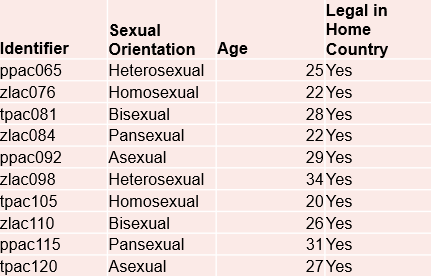
\includegraphics[width=.6\linewidth]{pseudonymization.png}
\end{figure}

\section{Ethics}

\colorbox{green}{Ethics} is\\
\bulletPoint Doing the “\colorbox{yellow}{right thing}” (subjective)\\
\bulletPoint behaving \colorbox{yellow}{professionally and responsibly}

\section{Diversity as Cyber Defense}

\colorbox{green}{Reddington’s Law};\\
“When you make things harder to access, you make them harder to access”\\
The more you \colorbox{yellow}{secure} things against ‘attackers’ the more you \colorbox{yellow}{reduce access} for
old people, poor people, disabled people.

Someone with multiple disabilities since birth, inability to speak, or
live independently, and can often be violent with frustration can be seen as a
walking zero-day exploit

\colorbox{green}{Disability} is \colorbox{pink}{context dependent} -  A wheelchair user is not disabled when playing chess. \\
\colorbox{pink}{long term systemic biases} might mean that access to these things is \colorbox{pink}{restricted}\\
(particularly if they cost money)

The question to ask is: \\
How is my product/company disabling/excluding people? \\
Or, hopefully, how is my product/company including people?

Hard to tell to what extent neurodivergence is diversity\\
there are now higher diagnosis rates and changes in definitions

The more similar all your employees are, the easier it is to write an ‘algorithm for business’\\
But if you treat all your employees the same, then every tiny difference will create a loophole,
many of them security flaws and your algorithm will be an inelegant mess of exceptions.

The \colorbox{pink}{more diverse} your company is, the \colorbox{pink}{more resilient} it is.\\
For every part of your business algorithm there is a disabled person who breaks it.

You need to think about how this affects security – both good and bad. \\
Every \colorbox{pink}{fix} you put in place on your business algorithm probably makes you \colorbox{pink}{better} for business continuity

E.g.,\\
\bulletPoint When your marketing staff have a lot of diversity, you are less likely to produce offensive messages.  \\
\bulletPoint If your sales team speaks nine languages, then you are going to be able to sell more stuff.\\
\bulletPoint If you are all using the same model laptop with the same software then the same bug will shut the company down.

Diversity is an \colorbox{yellow}{investment};\\
For any aspect of diversity, there is a business \colorbox{pink}{cost to improving it}.

Sometimes that’s just having a reasonable chat with a disabled person.\\
Sometimes it’s paying a premium in salary for diversity.\\
Sometimes it’s increasing the IT budget so they can cope with different types of equipment.

In extreme cases that cost might include having to sack a bunch of employees who can’t play nice. \\
But those employees were going to cost the company dearly pretty soon anyway.

Counterpoints;\\
\bulletPoint A simple business algorithm is much easier to write and run. \\
\bulletPoint Many of the accommodations you make for disabled people are easier at scale\\
– they can be disproportionately \colorbox{pink}{hard for microbusinesses}. \\
(i.e if you have two employees, increased absences from work can be really damaging)  \\
(the equality act 2010 recognises organization size as a factor) \\
\bulletPoint Change is really expensive: not just in money. \\
\bulletPoint It’s impossible (by definition) to accommodate all disabilities so why try?

Some companies are in \colorbox{green}{Diversity Theatre} - e.g., Pride Month

\chapter{Guest lecture - John Randell's daily tasks}

Daily tasks;\\
\bulletPoint Footprints tickets\\
\bulletPoint ‘Risky sign ins’\\
\bulletPoint SentinelOne (malicious/suspicious files and disabled agents)\\
\bulletPoint Microsoft Defender - links in emails clicked that are deemed risky, email thresholds, risky users\\
\bulletPoint Emails reported to CyberSec - 1000\textless emails reported over month\\
- 10\% of them phishing emails that should have been blocked\\
\bulletPoint National Cyber Security Centre quarantined emails\\
\bulletPoint Audit Outlook rules and email forwarding

\section{Footprints tickets}

Need to \colorbox{yellow}{ask / answer} the following for many people;\\
Is this a phishing email?\\
Why is x being blocked?\\
Missing student\\
Can this shared emailbox be deleted?\\
I’m being spammed!

\section{‘Risky sign ins’}

What makes a sign in risky?\\
\bulletPoint \textbf{IP address} – has a \colorbox{yellow}{poor ip quality} score rating or \colorbox{yellow}{reported malicious activity}.\\
\bulletPoint Different \textbf{metadata} (\colorbox{yellow}{inconsistent} browser and version, device, location)\\
\bulletPoint \textbf{MFA} \colorbox{yellow}{not enabled} (rare now)\\
\bulletPoint MFA \colorbox{yellow}{previously fulfilled} (\textbf{cookies})\\
\bulletPoint \textbf{Inactive} account getting \colorbox{yellow}{login events}\\
\bulletPoint Certain \textbf{applications} being accessed by \colorbox{yellow}{non IT users}

Solution Number within last month;\\
\bulletPoint No further action: 99 \\
\bulletPoint User sessions revoked: 47 \\
\bulletPoint Leaver; disabled account: 19\\
\bulletPoint It ticket raised: 15 \\
\bulletPoint No MFA set up: 3 \\
\bulletPoint Staff compromised credentials: 1 \\
\bulletPoint Staff VPN use (unsuccessful logins): 1

How to tell what the solution is?\\
\colorbox{green}{Azure} Risky sign ins - \colorbox{yellow}{logs}

\begin{figure}[H]
  \centering
  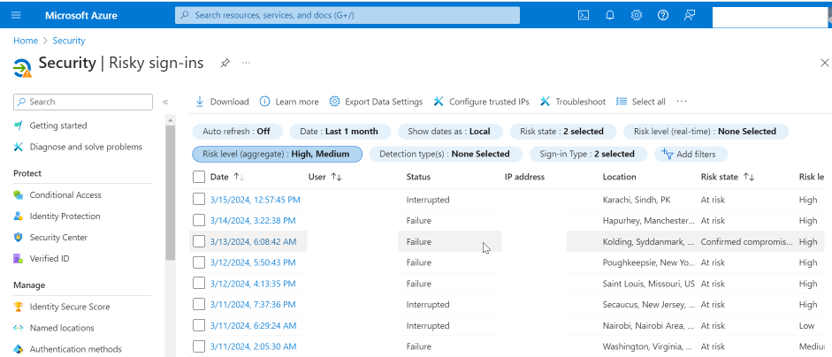
\includegraphics[width=\linewidth]{azure sign ins.png}
\end{figure}

\begin{figure}[H]
  \centering
  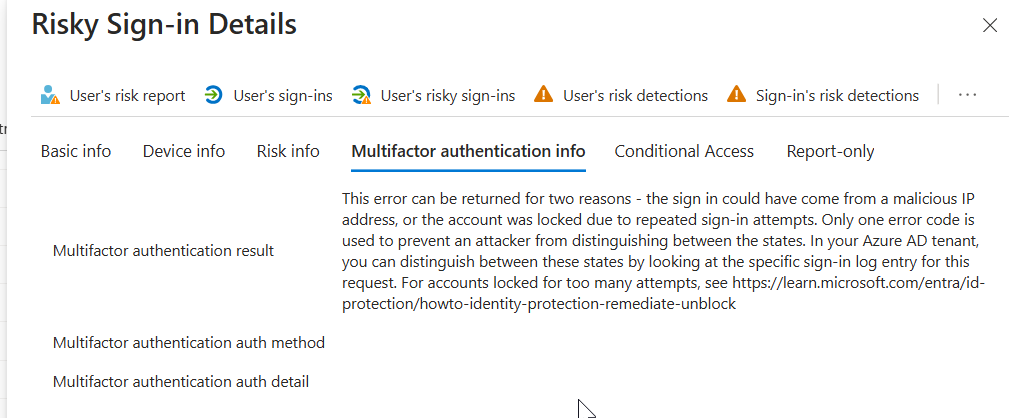
\includegraphics[width=\linewidth]{azure risky sign ins.png}
\end{figure}

You can use \colorbox{yellow}{databases} for IP quality scores\\
\url{Ipqualityscore.com}, \url{abuseipdb.com}

\begin{figure}[H]
  \centering
  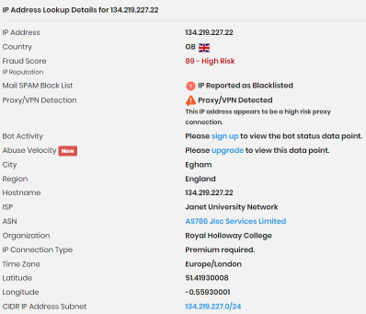
\includegraphics[width=.6\linewidth]{IP quality score.png}
\end{figure}

\section{SentinelOne}

The College’ uses \colorbox{green}{SentinelOne} as the \colorbox{green}{endpoint management system}. \\
We also have a \colorbox{yellow}{service provider} that \colorbox{yellow}{monitors alerts 24/7}

It uses \colorbox{yellow}{machine learning} for monitoring personal computers, servers\\
Uses \colorbox{yellow}{heuristics behavioural AI} to look for behaviours\\
Looks up against \colorbox{yellow}{database} virustotal

Endpoint protection;

\begin{figure}[H]
  \centering
  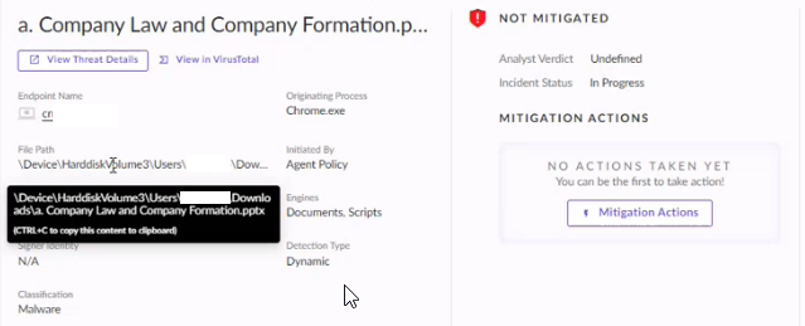
\includegraphics[width=.6\linewidth]{endpoint protection.png}
\end{figure}

\section{Microsoft Defender}

\begin{figure}[H]
  \centering
  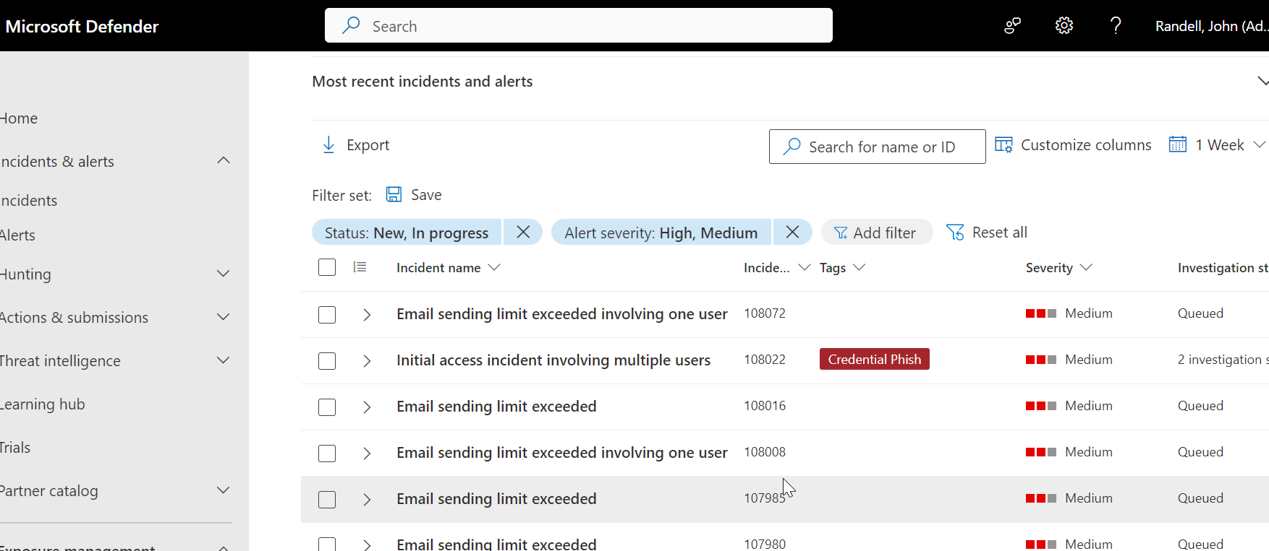
\includegraphics[width=\linewidth]{Microsoft defender.png}
\end{figure}

\bulletPoint Another source of risky sign ins / compromised accounts\\
\bulletPoint Can see \colorbox{yellow}{risky clicks} from emails giving ideas of suggested phishing\\
\bulletPoint Email \colorbox{yellow}{limits} for those who send lots of emails.\\
\bulletPoint Anonymous tokens (for identification)

\newpage

\section{Emails reported}

User \colorbox{yellow}{submissions};

\begin{figure}[H]
  \centering
  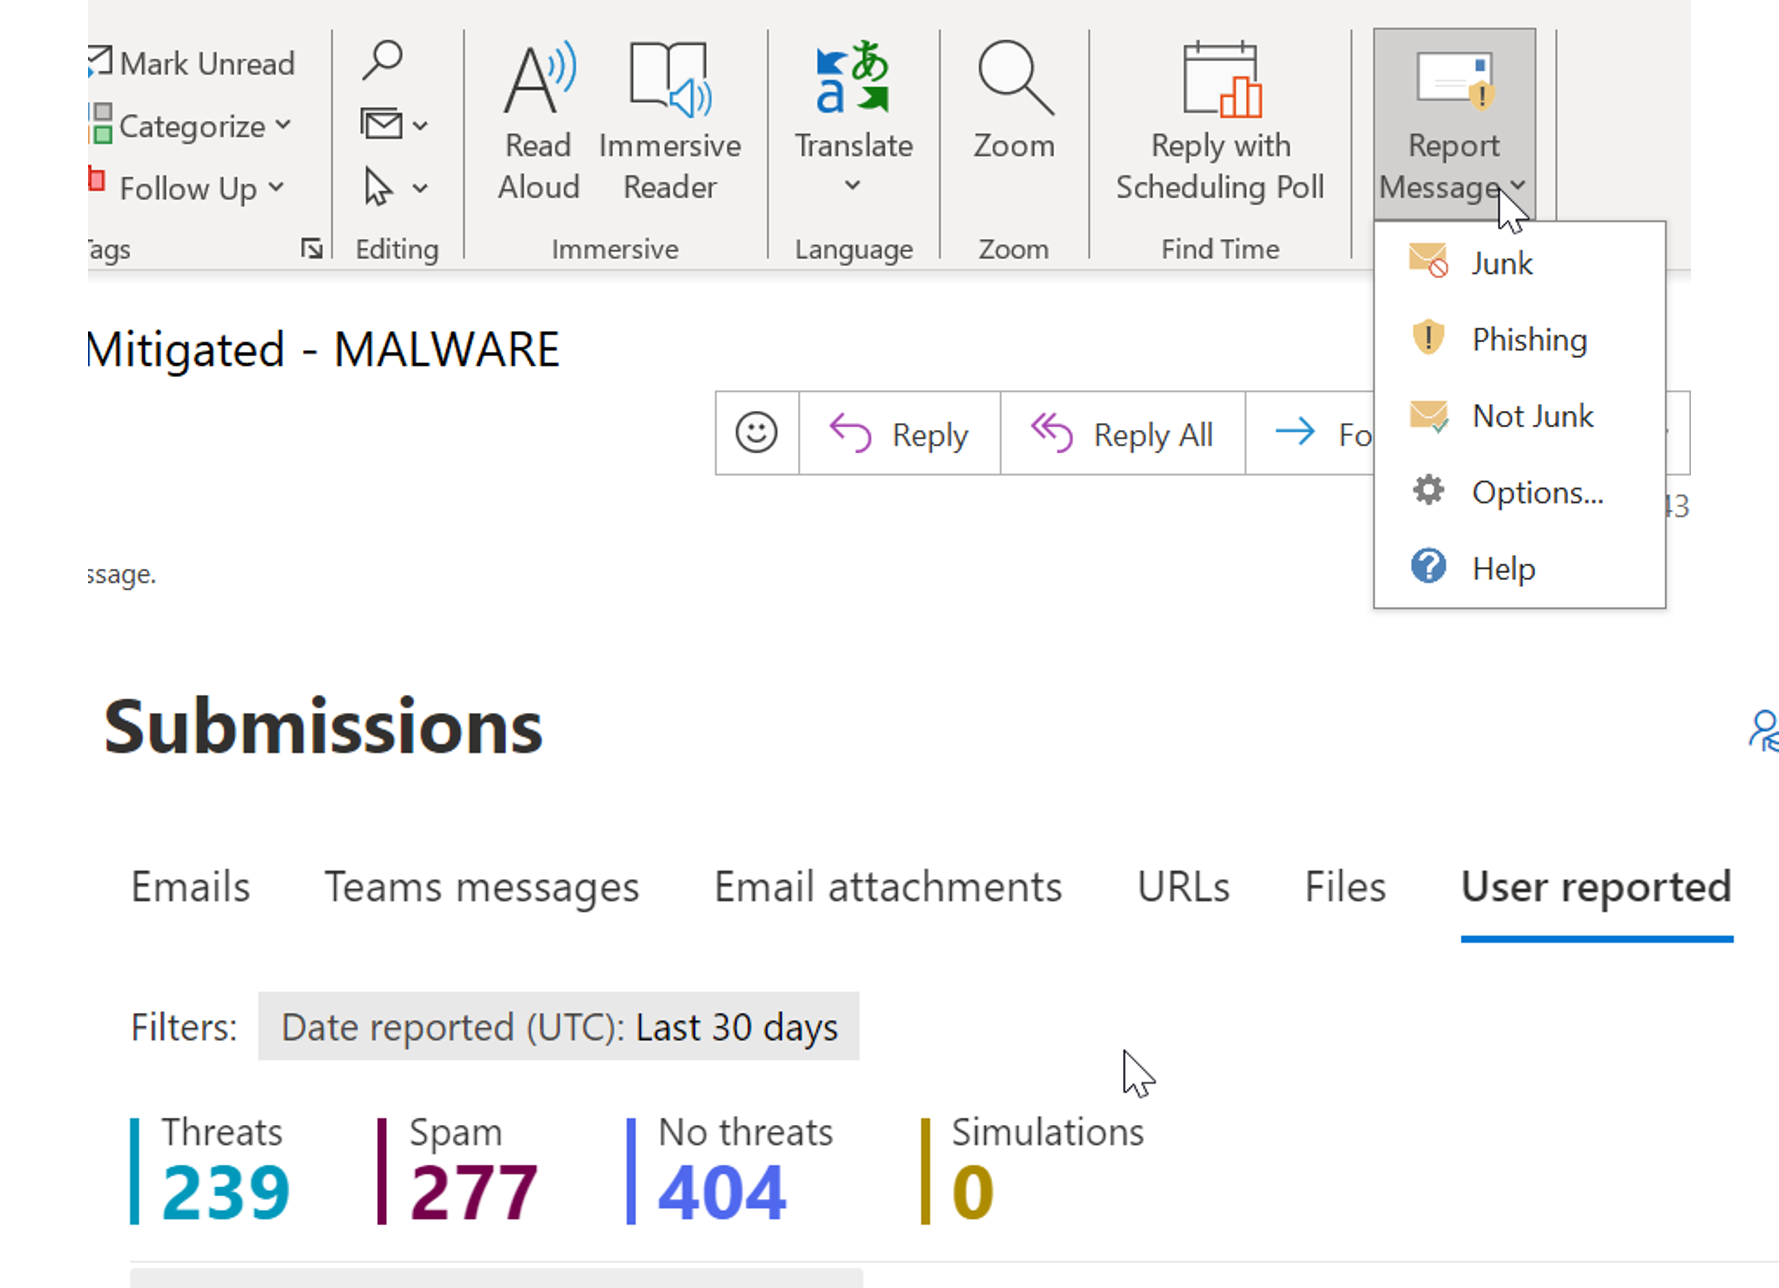
\includegraphics[width=.6\linewidth]{user submissions.png}
\end{figure}

Can analyse attached email in \colorbox{green}{phishtool}

\begin{figure}[H]
  \centering
  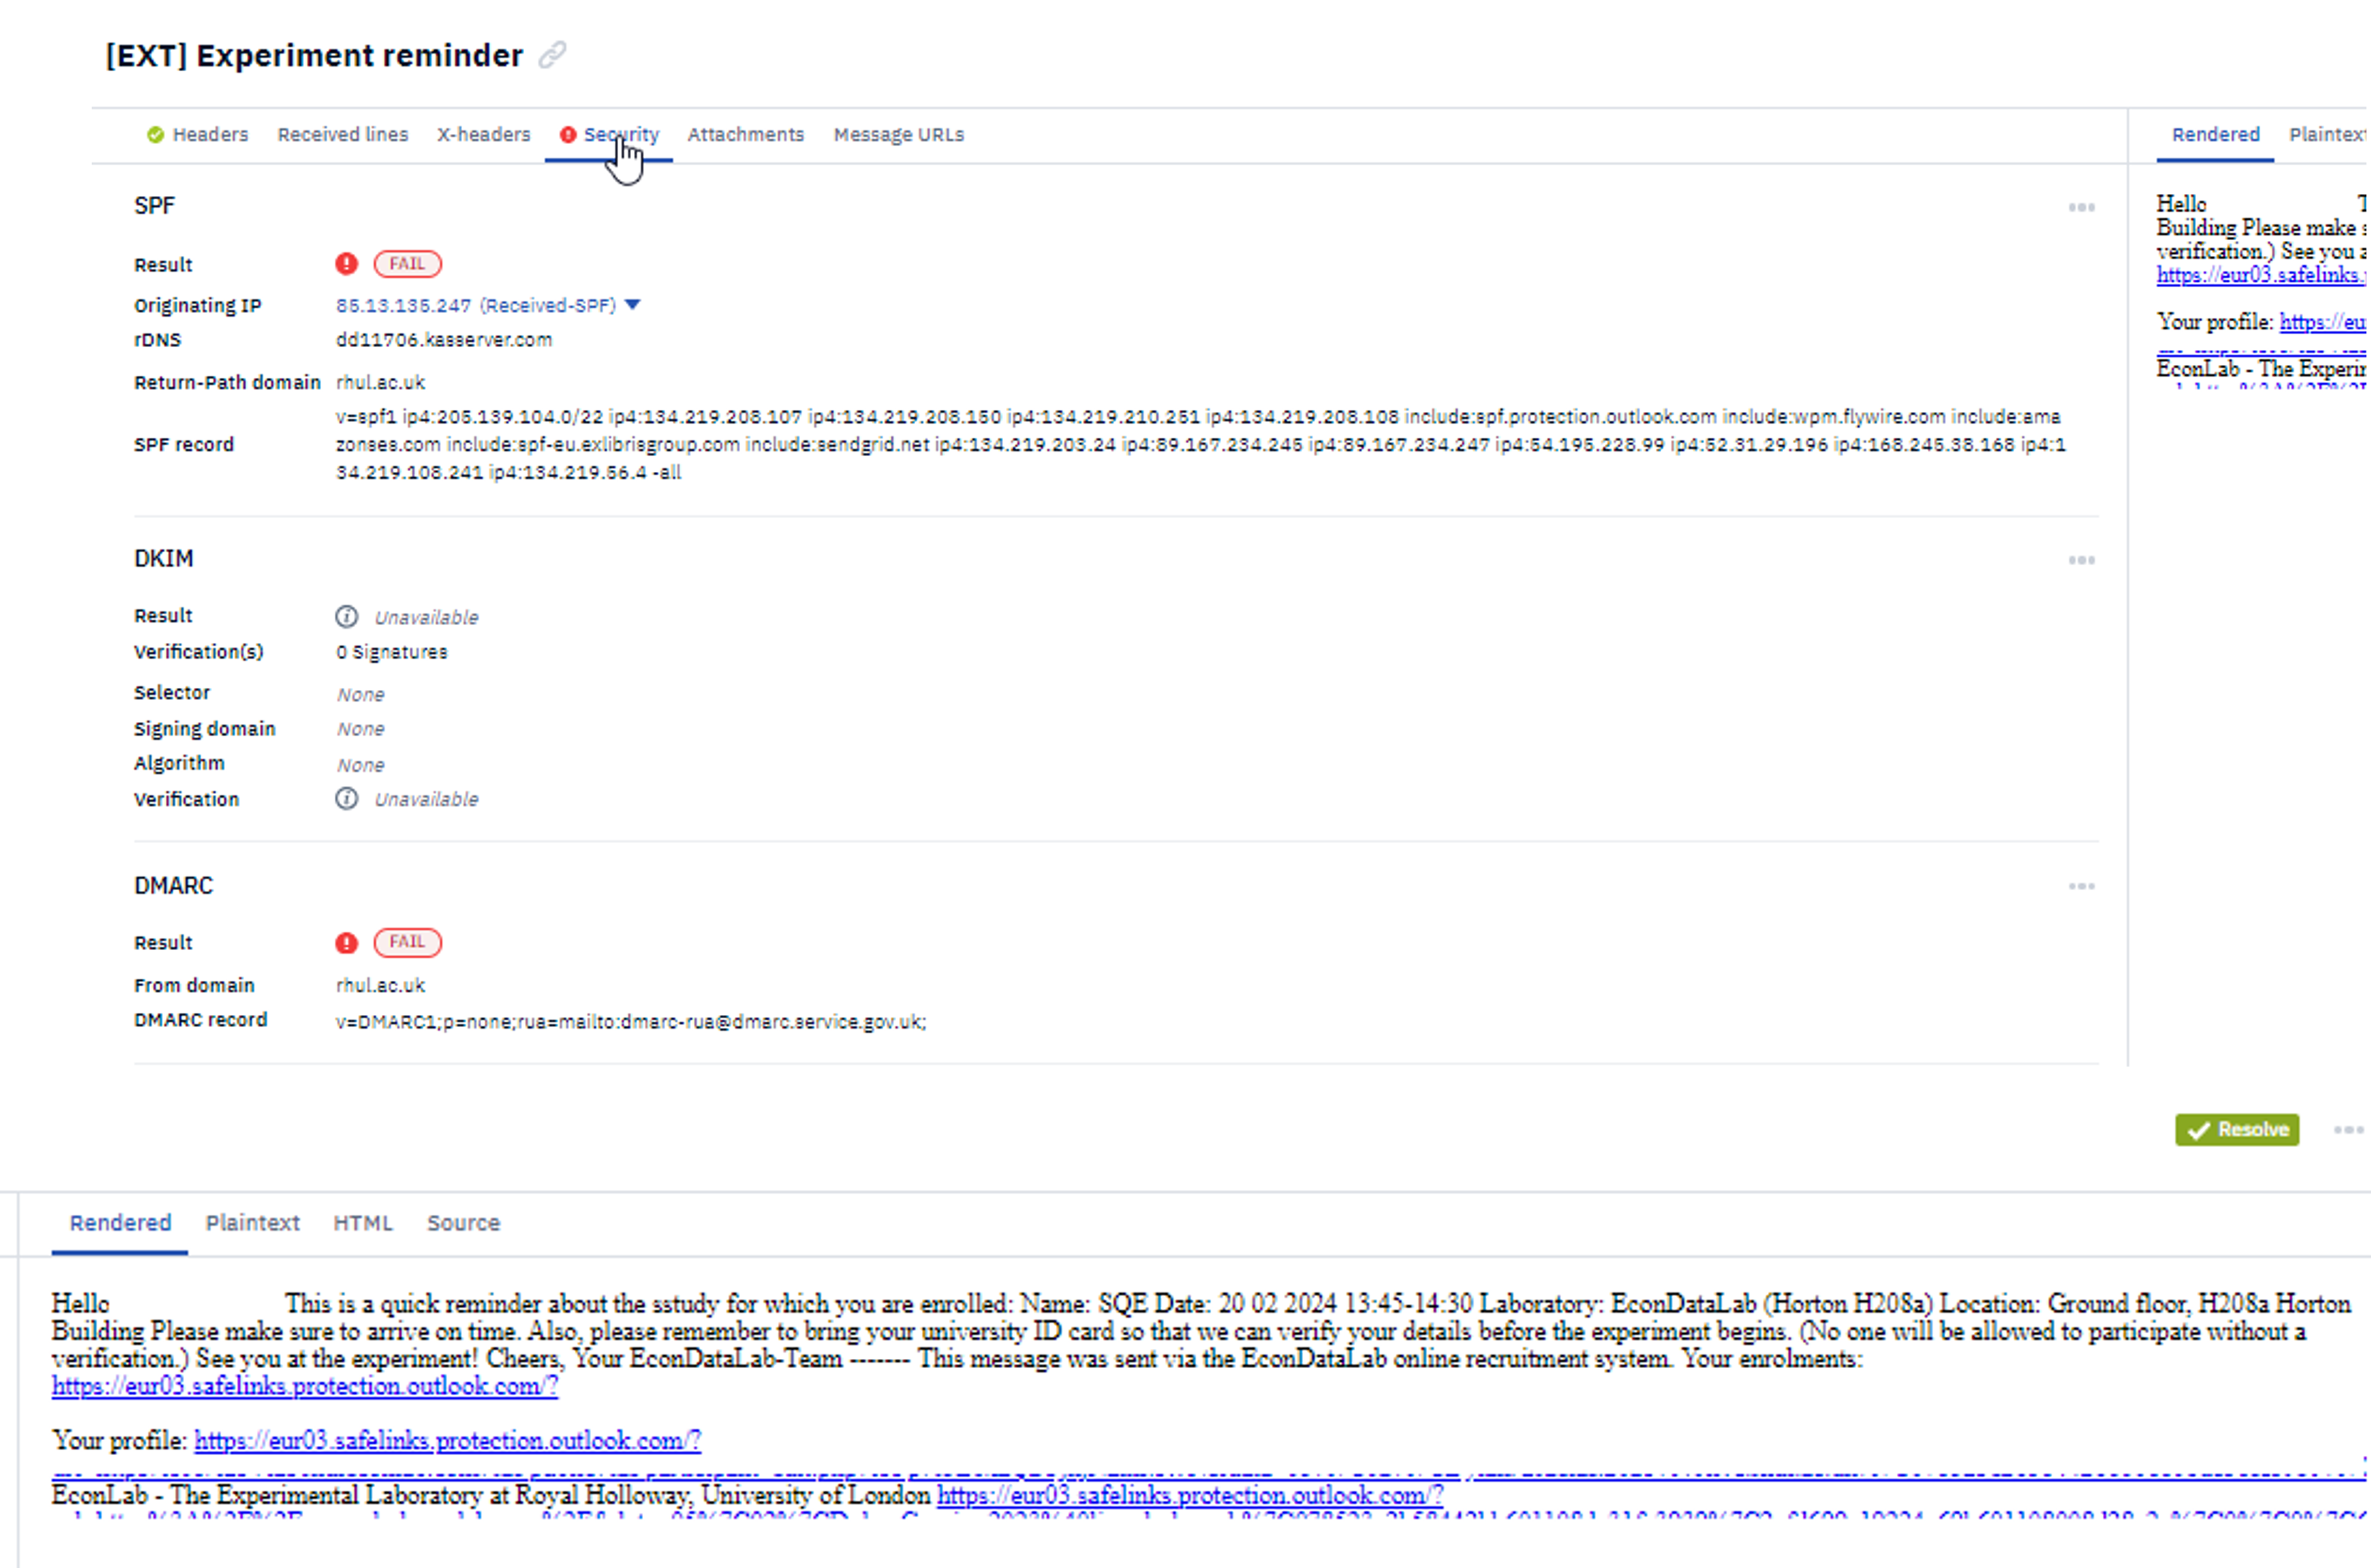
\includegraphics[width=\linewidth]{phishtool.png}
\end{figure}

\colorbox{green}{SPF} stands for Sender Policy Framework.\\
It allows you to \colorbox{yellow}{cache a list of authorized IP} addresses that are allowed to
\colorbox{yellow}{send emails to your} \colorbox{yellow}{customers} on your behalf

\colorbox{green}{DKIM} stands for Domain Keys Identified Mail.\\
DKIM is a \colorbox{pink}{stronger authentication method} than SPF since it uses \colorbox{pink}{public-key
  cryptography} instead of IP addresses. Sender can attach DKIM signatures to
email headers and \colorbox{yellow}{validate} them using a public cryptographic key
found in the company's DNS record.

\colorbox{green}{DMARC} is a \colorbox{yellow}{combination} of DKIM and SPF

\section{Quarantined emails}

Lots of DMARC fail = bad\\
\bulletPoint Someone spoofing emails\\
\bulletPoint Someone sending malicious links through a compromised account.

\begin{figure}[H]
  \centering
  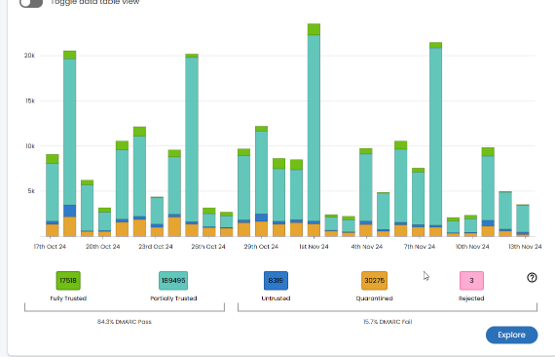
\includegraphics[width=\linewidth]{lots of DMARC.png}
\end{figure}

\section{Audit Outlook rules and email forwarding}

\colorbox{pink}{Looking through csv is hard}, tiring, etc.\\
Use a little AI

\begin{figure}[H]
  \centering
  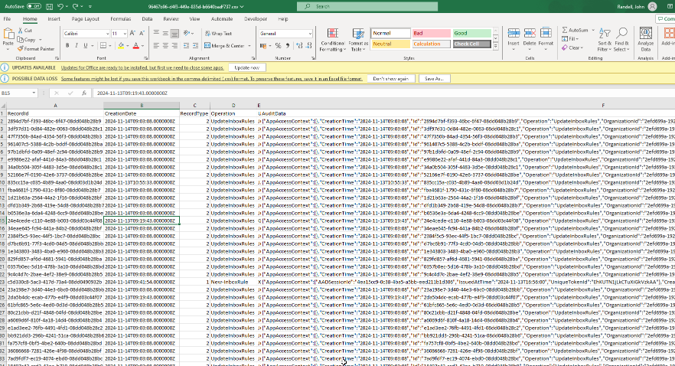
\includegraphics[width=\linewidth]{Audit Outlook rules and email forwarding 1.png}
  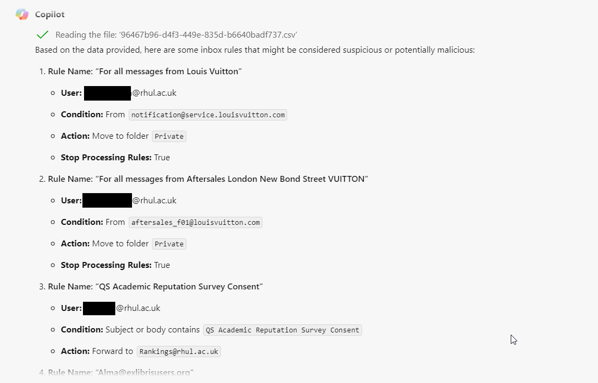
\includegraphics[width=\linewidth]{Audit Outlook rules and email forwarding 2.png}
\end{figure}

\chapter{Unit 8 - Staff Management}

This is \colorbox{yellow}{Human resources security}

“By far the \colorbox{pink}{most common} [reported] type of breach or attack is \colorbox{pink}{phishing} (84\% of businesses and 83\% of charities)”

“\colorbox{pink}{over 95 percent} of all incidents investigated recognize \colorbox{pink}{“human error”} as a contributing factor. The most
commonly recorded form of human errors include system misconfiguration, poor patch management, use of
default user names and passwords or easy-to-guess passwords, lost laptops or mobile devices, and
disclosure of regulated information via use of an incorrect email address.”

\colorbox{yellow}{Recruitment and training are vital} pieces of the security algorithm.\\
To be good at this you will need to \colorbox{pink}{develop people skills}.

The ISO standards recognise that people are important with eight controls.  \\
Note that this doesn’t include things that are already business functions: “doing what you are told”

The controls can be organised into three groups.\\
\hphantom{12}Before employment\\
\hphantom{1234}6.1 Screening\\
\hphantom{1234}6.2 Terms and conditions of employment\\
\hphantom{12}During employment\\
\hphantom{1234}6.3 Information security awareness, education, and training\\
\hphantom{1234}6.4 Disciplinary process\\
\hphantom{1234}6.6 Confidentiality or non-disclosure agreements\\
\hphantom{1234}6.7 Remote working\\
\hphantom{1234}6.8 Information security event reporting\\
\hphantom{12}At the end of employment. \\
\hphantom{1234}6.5 Responsibilities after termination or change of employment

\section{Before Employment}

E.g., new Judo Club\\
Judo is quite dangerous: you need to trust everybody in the room implicitly\\
\colorbox{yellow}{How do they check if I am safe} and competent without being insulting to a potential new member?\\
How is it different based on experience?

\newpage

\subsection{6.1 Screening}

There are \colorbox{cyan}{five basic checks}:\\
\bulletPoint Character References\\
\bulletPoint CV \\
\bulletPoint Academic and Professional Qualifications\\
\bulletPoint Identity Check\\
\bulletPoint Credit Check/Criminal Records check\\
Often also includes ‘right to live and work in the country’

Eligible convictions or cautions become '\colorbox{green}{spent}' after a specified period of
time, known as the 'rehabilitation period', allowing offenders to '\colorbox{yellow}{wipe their slate clean}'.

There are \colorbox{cyan}{four levels} of Criminal Records Check in the UK. (it’s called DBS) \\
1. a basic check, which shows \colorbox{yellow}{unspent} convictions and conditional cautions\\
2. a standard check, which shows \colorbox{yellow}{spent and unspent} convictions and cautions\\
3. an enhanced check, which shows the same as a standard check plus any
\colorbox{yellow}{information held by} \colorbox{yellow}{local police} that’s considered relevant to the role\\
4. an enhanced check with \colorbox{yellow}{barred lists}, which shows the same as an enhanced
check plus whether the applicant is on the list of people barred from doing the role

DBS Checks \colorbox{pink}{don’t} (generally) \colorbox{pink}{include crimes overseas}. \\
Employers can run a DBS basic \colorbox{pink}{check on any employee}.\\
\colorbox{pink}{More detailed checks} can only be done for specific jobs.  This includes: \\
\bulletPoint Healthcare \\
\bulletPoint Childcare \\
\bulletPoint Regulated professions (accountants, vets, senior management\\
\bulletPoint Firearms dealer\\
\bulletPoint etc.

A criminal records check \colorbox{pink}{isn’t a ‘yes/no’}. E.g., Timpson\\
Timpson in the UK employees a lot of former criminals (10\% of total staff). \\
They have their own rules:\\
\bulletPoint No sexual offenses\\
\bulletPoint Over 25 \\
\bulletPoint “Most colleagues committed acquisitive or drug-related offences,
and are often from a care background” (relationship project)\\
This is an example of a company being explicit about how they treat screening.

\subsection{6.2 Terms and conditions of employment}

Every \colorbox{yellow}{job description should include} a statement saying the employee will \colorbox{yellow}{abide by the} \colorbox{yellow}{security policy}. \\
\colorbox{pink}{Some} roles will \colorbox{pink}{require specific} security requirements

You will have to \colorbox{yellow}{review all roles} first to \colorbox{yellow}{work out which roles have which requirements}. \\
If the policy says ‘make sure assets are secure’, (some) job descriptions also say ‘make sure assets are secure’

Employment \colorbox{cyan}{contracts should}:\\
\bulletPoint \colorbox{yellow}{Reflect} the organisation’s \colorbox{yellow}{policies} for information security\\
\bulletPoint State that anyone given access to confidential information should sign an \colorbox{yellow}{NDA} prior to being given access\\
\bulletPoint State employee’s \colorbox{yellow}{legal responsibilities and rights}, for example regarding copyright or data protection\\
\bulletPoint State employee’s responsibilities for \colorbox{yellow}{information classification}\\
\bulletPoint State employee’s  responsibilities for the \colorbox{yellow}{handling} of information \colorbox{yellow}{from third parties}\\
\bulletPoint State the \colorbox{yellow}{actions} that will be taken if anyone \colorbox{yellow}{ignores security rules}

\section{During Employment}

In general, all of these controls are quite linked together

\subsection{6.4 Disciplinary process}

The company \colorbox{pink}{should already have a disciplinary process}

“Clearly no disciplinary process can start until the existence of a breach
has been verified” (Calder and Watkins) - not completely true

'A disciplinary process should be \colorbox{yellow}{formalized and communicated} to take actions
against personnel and other relevant interested parties who have committed
an information security policy violation.'

Can I sack this person? \colorbox{pink}{Arguable} if this is \colorbox{pink}{necessary}\\
everything would normally be covered under normal disciplinary context.

'\colorbox{pink}{Business requirements} as well as other factors as required. The
disciplinary process should also be used as a \colorbox{yellow}{deterrent} to prevent personnel
and other relevant interested parties from violating the information security
policy, topic-specific policies, and procedures for information security.
Deliberate information security policy violations \colorbox{pink}{can require immediate actions}.'

From this quote, it becomes clear: this is talking about policy violations rather than breaches. \\
There should be a process for punishing workers if they violate a policy \colorbox{yellow}{even if it causes no harm}.

In practice this looks like:\\
“If you click on the test phishing email IT sent, then you have to go a training
on Cybersecurity for three hours on Friday. It’s on-site.”\\
(HR infringements are often dealt with in the same way)

\subsubsection{Implementation guidance}

Your entire ISMS is irrelevant if staff don’t follow the rules\\
\colorbox{pink}{Senior staff are a particular problem}

The \colorbox{pink}{simpler} the polices are, the \colorbox{pink}{easier} they are to remember, understand and follow. \\
You need to have a full and complete answer to any “Why” questions.

Process should \colorbox{yellow}{ensure correct and fair treatment} for employees suspected of breaching security

Process should allow a graduated \colorbox{yellow}{response, depending on nature of breach},
impact on business, whether a first offence, whether violator was
properly trained, relevant laws, etc

\subsection{6.6 Confidentiality}

'Confidentiality or non-disclosure agreements reflecting the organization's
needs for the protection of information should be identified, documented,
regularly reviewed and signed by personnel and other relevant interested parties.'

What percentage of NDAs are broken? \\
We don’t know, but over 25\% of jurors talk about cases with family and friends.

\colorbox{pink}{NDAs require a lot of money to enforce}. They tend to be very ‘security theatre’\\
Arguably your position as Cyber Security people is to get it signed and
leave it to the lawyers

\colorbox{green}{Security theater} is the practice of \colorbox{yellow}{implementing security measures} that are
considered to provide the \colorbox{yellow}{feeling of improved security} while \colorbox{yellow}{doing little} or
nothing to achieve it.

The term has been  widely adopted by the media and the public, particularly in
discussions surrounding the Transportation Security Administration.

Security Theatre is \colorbox{pink}{valid as a marketing tool}; e.g., selling fake cctv cameras\\
But your \colorbox{pink}{staff need to know what the difference is}. \\
Also; don’t let it come out of your budget!

\subsection{6.3 Information security awareness, education, and training}

Teaching is hard - not everybody likes learning stuff\\
Training is useless if senior staff are not good examples. \\
\colorbox{pink}{Culture beats training every time}.

\colorbox{yellow}{Anyone with access} to corporate information should receive some information security \colorbox{yellow}{training} \\
\colorbox{pink}{Level required will depend} on their role and level of access to information

Training should be sufficient to ensure the individual can carry out security
procedures and understands how to use systems securely

Training should \colorbox{yellow}{always include coverage of the acceptable use policy}

\subsection{6.7 Remote working}

Often a question of “What do my customers/suppliers require?”

CampusAnywhere limits many resources only to students. \\
\colorbox{pink}{Email is a very big factor here}.

\subsection{6.8 Information Security Event Reporting}

'The organization should provide a \colorbox{yellow}{mechanism} for personnel to \colorbox{yellow}{report} observed
or suspected information security events through appropriate channels in a \colorbox{yellow}{timely manner}.'

Must be extremely simple:\\
Who do you call? \\
What do you call them about?

Multiple channels: an email address, a phone number, and a physical person in the office\\
“Hey Jude, is this meant to happen?”

\section{After Employment}

\subsection{6.5 Responsibilities after termination or change of employment}

There are some other relevant controls “Removal of Access”, “Return of Assets”

There \colorbox{yellow}{should be a named person in charge} of removing access from people who leave. \\
That named person should have a checklist.

Colonial Pipeline hack/breach was from someone not removing old VPN accounts.\\
People who are leaving are less under your influence.

\chapter{Unit 9 - Audit}

\section{Definitions}

Traditional definition of audit;\\
1. \textbf{An \colorbox{yellow}{examination} of an account} or of accounts, with a \colorbox{yellow}{hearing} of the parties
concerned, by proper officers, or persons appointed for that purpose, who
\colorbox{yellow}{compare the charges} with the vouchers, examine witnesses, and state the balance. \\
2. \textbf{The \colorbox{yellow}{result} of such an examination}, or account as \colorbox{yellow}{adjusted} by auditors; a final account.

To examine \textbf{and adjust} an account or accounts, by proper officers, or by persons
legally authorized for the purpose.

These definitions have broadened over time;\\
1. \textbf{Check of accounts}: a formal examination, correction, and official endorsing
of financial accounts, especially those of a business, undertaken annually by an accountant \\
2. \textbf{Efficiency check}: a systematic check or assessment, especially of the
efficiency or effectiveness of an organization or department, typically carried
out by an independent assessor

Modern definition of audit;\\
\colorbox{green}{Audits} provide \colorbox{yellow}{third-party assurance} to various stakeholders that the \colorbox{yellow}{subject matter} is
\colorbox{yellow}{free} \colorbox{yellow}{from material misstatement}.

The term is \colorbox{pink}{most frequently} applied to audits of the \colorbox{pink}{financial} information relating to a legal person. \\
Other commonly audited areas include secretarial and compliance, internal controls, quality management, project management, …

As a result of an audit, stakeholders may \colorbox{pink}{evaluate and improve} the effectiveness
of \colorbox{pink}{risk} \colorbox{pink}{management, control, and governance} over the subject matter.

\colorbox{green}{Internal} audits;\\
\bulletPoint Conducted by internal staff or a dedicated internal audit team.\\
\bulletPoint Evaluate internal controls, processes, and risk management.\\
\bulletPoint Continuous or periodic.\\
\bulletPoint Focused on improvement and risk mitigation.\\
\bulletPoint Reports to management and board of directors

\colorbox{green}{External} Audits;\\
\bulletPoint Conducted by independent, external auditors.\\
\bulletPoint Provide an objective opinion on financial statements or compliance.\\
\bulletPoint Typically annual.\\
\bulletPoint Ensures statutory or regulatory compliance.\\
\bulletPoint Reports to shareholders, regulators, or other external stakeholders.

\begin{figure}[H]
  \centering
  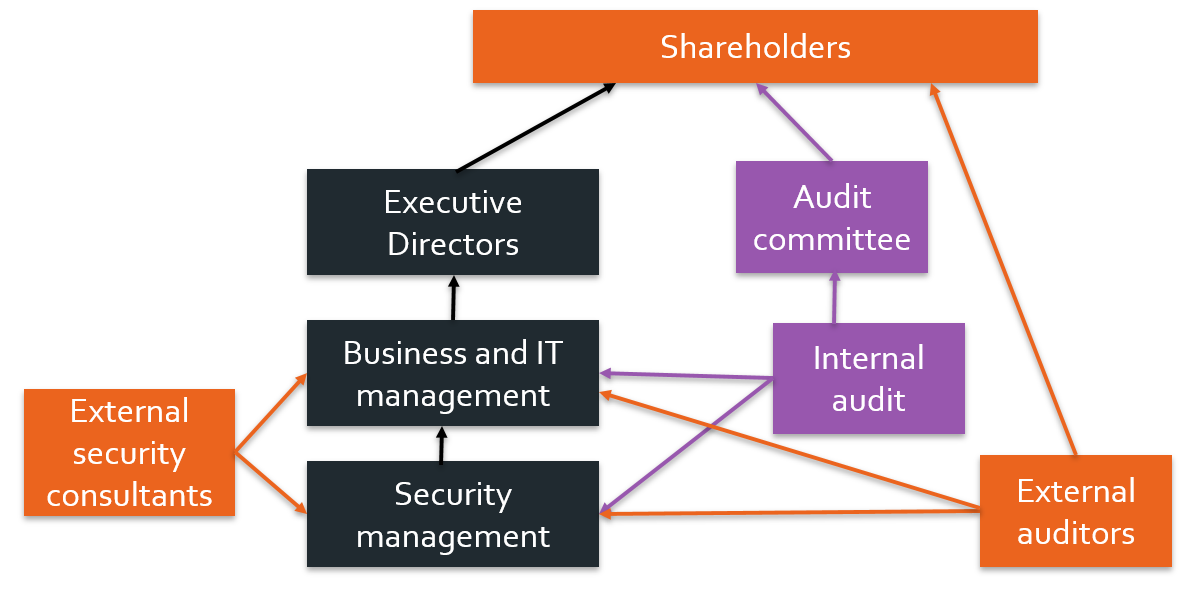
\includegraphics[width=\linewidth]{governance structures and accountability.png}

  Governance structures and accountability
\end{figure}

\section{Audits and Risk}

How does an audit (or any type) impact your ability to make money?

Cons;\\
\bulletPoint Audits are \colorbox{pink}{expensive} in both time and money \\
\bulletPoint Audits are extremely expensive if you are purposely doing something wrong. \\
\bulletPoint If you are doing everything \colorbox{pink}{correctly}, audits \colorbox{pink}{don’t tell you anything useful}. (not necessarily)

Pros;\\
\bulletPoint It’s \colorbox{pink}{easy to reassure clients} \\
\bulletPoint You can \colorbox{pink}{trust} your internal processes more\\
\bulletPoint You know the \colorbox{pink}{extent} of your exposure (legal, technical)

Risk compensation (\colorbox{green}{Risk homeostasis}) - The Psychology of Risk Taking Behavior\\
“In a Munich study, part of a fleet of taxicabs were equipped with anti-lock
brakes (ABS), while the remainder had conventional brake systems. In other
respects, the two types of cars were identical. The crash rates, studied over
three years, were a little higher for the cabs with ABS”

In a business, this is quite rational\\
if you \colorbox{yellow}{know there is less risk} in one area, then you can \colorbox{yellow}{take more risks} in
another area and \colorbox{yellow}{hopefully make more money}.

\newpage

\section{How would you do an audit?}

Could audit;\\
\bulletPoint Email hygiene\\
\bulletPoint Network logs \\
\bulletPoint Patch management \\
\bulletPoint Access control \\
\bulletPoint Training \\
\bulletPoint Penetration testing

\subsection{The ISO 27001 Audit}

An audit is \colorbox{pink}{generally negative}:\\
“you didn’t do this” rather than positive “You are great at this”

The \colorbox{cyan}{outcome} of an audit is normally:\\
\bulletPoint a written report\\
\bulletPoint a set of corrective actions and timeframes

\colorbox{green}{ISO 9001} is “\colorbox{yellow}{Have you documented everything}, is there an algorithm for everything?”\\
Lots of people hate it\\
Lots of computer people think it’s reasonable

It needs to be audited \\
No point having separate companies audit ISO9001 and ISO27001: \colorbox{yellow}{choose a company that can} \colorbox{yellow}{do both}.

There are two stages to an \colorbox{green}{ISO 27001 Audit}: \\
In the first stage the algorithm is checked to see if it is \colorbox{yellow}{consistent with ISO27001}. \\
In the second, longer, stage, the algorithm is checked to see if it’s \colorbox{yellow}{consistent with reality}. \\
Can be up to three months between stages.

There is a corporate \colorbox{pink}{tendency to adopt certifications for appearance} rather than substance.\\
"I'm putting you in charge of getting our 'ISO 9000' certification, We don't know what it is, but it looks great on brochures."

\colorbox{yellow}{Quality} of internal processes is \colorbox{yellow}{not reflected} in having the certification;\\
A customer saying, "Your product looks good, but you can't be our supplier unless your company is ISO 9000 certified."\\
The boss responds, "So... you don't care how bad our internal processes are, as long as they're well-documented and used consistently?"\\
The customer replies, "That's right."\\
The boss humorously concludes, "Our documented process says I must now laugh in your face and double our price."

Some don't "Actually improving cyber defense"\\
a preference for avoiding the real, hard work of bolstering cybersecurity measures.

while approving "Getting ISO 27001," \\
focus on obtaining certifications for appearance or compliance rather than
implementing substantive security improvements.

Some Organizations prioritize certification (e.g., ISO 27001) over genuinely
strengthening their cybersecurity posture.

There is a \colorbox{pink}{perception} that
some \colorbox{pink}{companies focus on check-the-box} compliance rather than meaningful change.\\

There are \colorbox{pink}{no required controls}\\
\colorbox{pink}{Skepticism} around \colorbox{pink}{relying solely on certifications} like
ISO 27001 or SOC2, suggesting that these may not guarantee robust security
practices without the implementation of real controls. There is a \colorbox{pink}{superficial
  reliance on documentation} instead of focusing on actual
security measures.

\colorbox{pink}{Professionals}, e.g., on linkedIn, also \colorbox{pink}{advertise the certs.} describing its benefits\\
While ISO 27001 can deliver the benefits described, it is very possible
for an organization to implement it poorly or superficially, resulting
in little to no real improvement in security or culture.

\end{document}
\end{article}